% Appendix B *** Appendix for chapter 6 now, labels remain "chapter 5" and "appendix B"

\chapter{Supplementary Data for Chapter 6}\label{AppendixB}
\lhead{Appendix C. \emph{Supplementary Data for Chapter 6}}

\begin{figure}[htp]
\centering
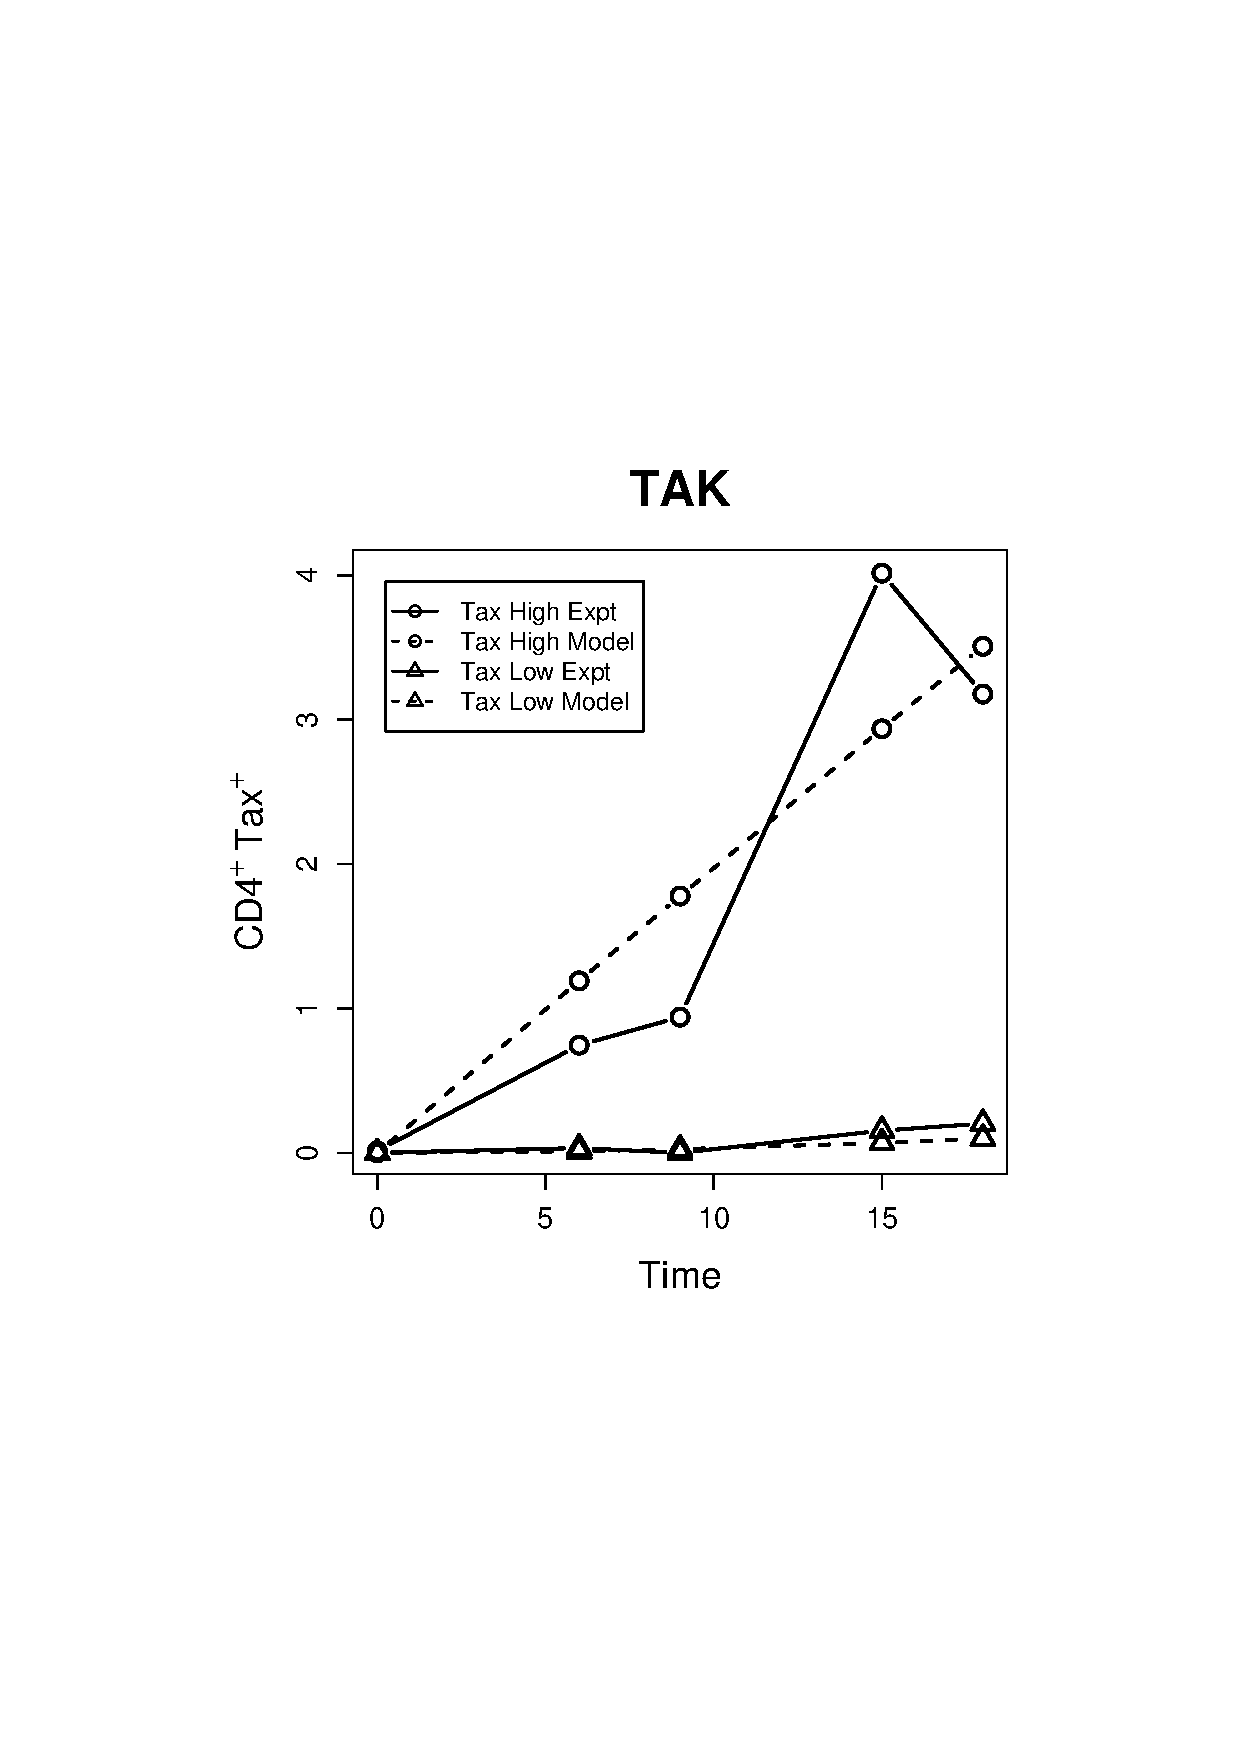
\includegraphics[width=7cm]{./Figures/chapter5/figure_timecourse_tak}%
\hspace{0cm}%
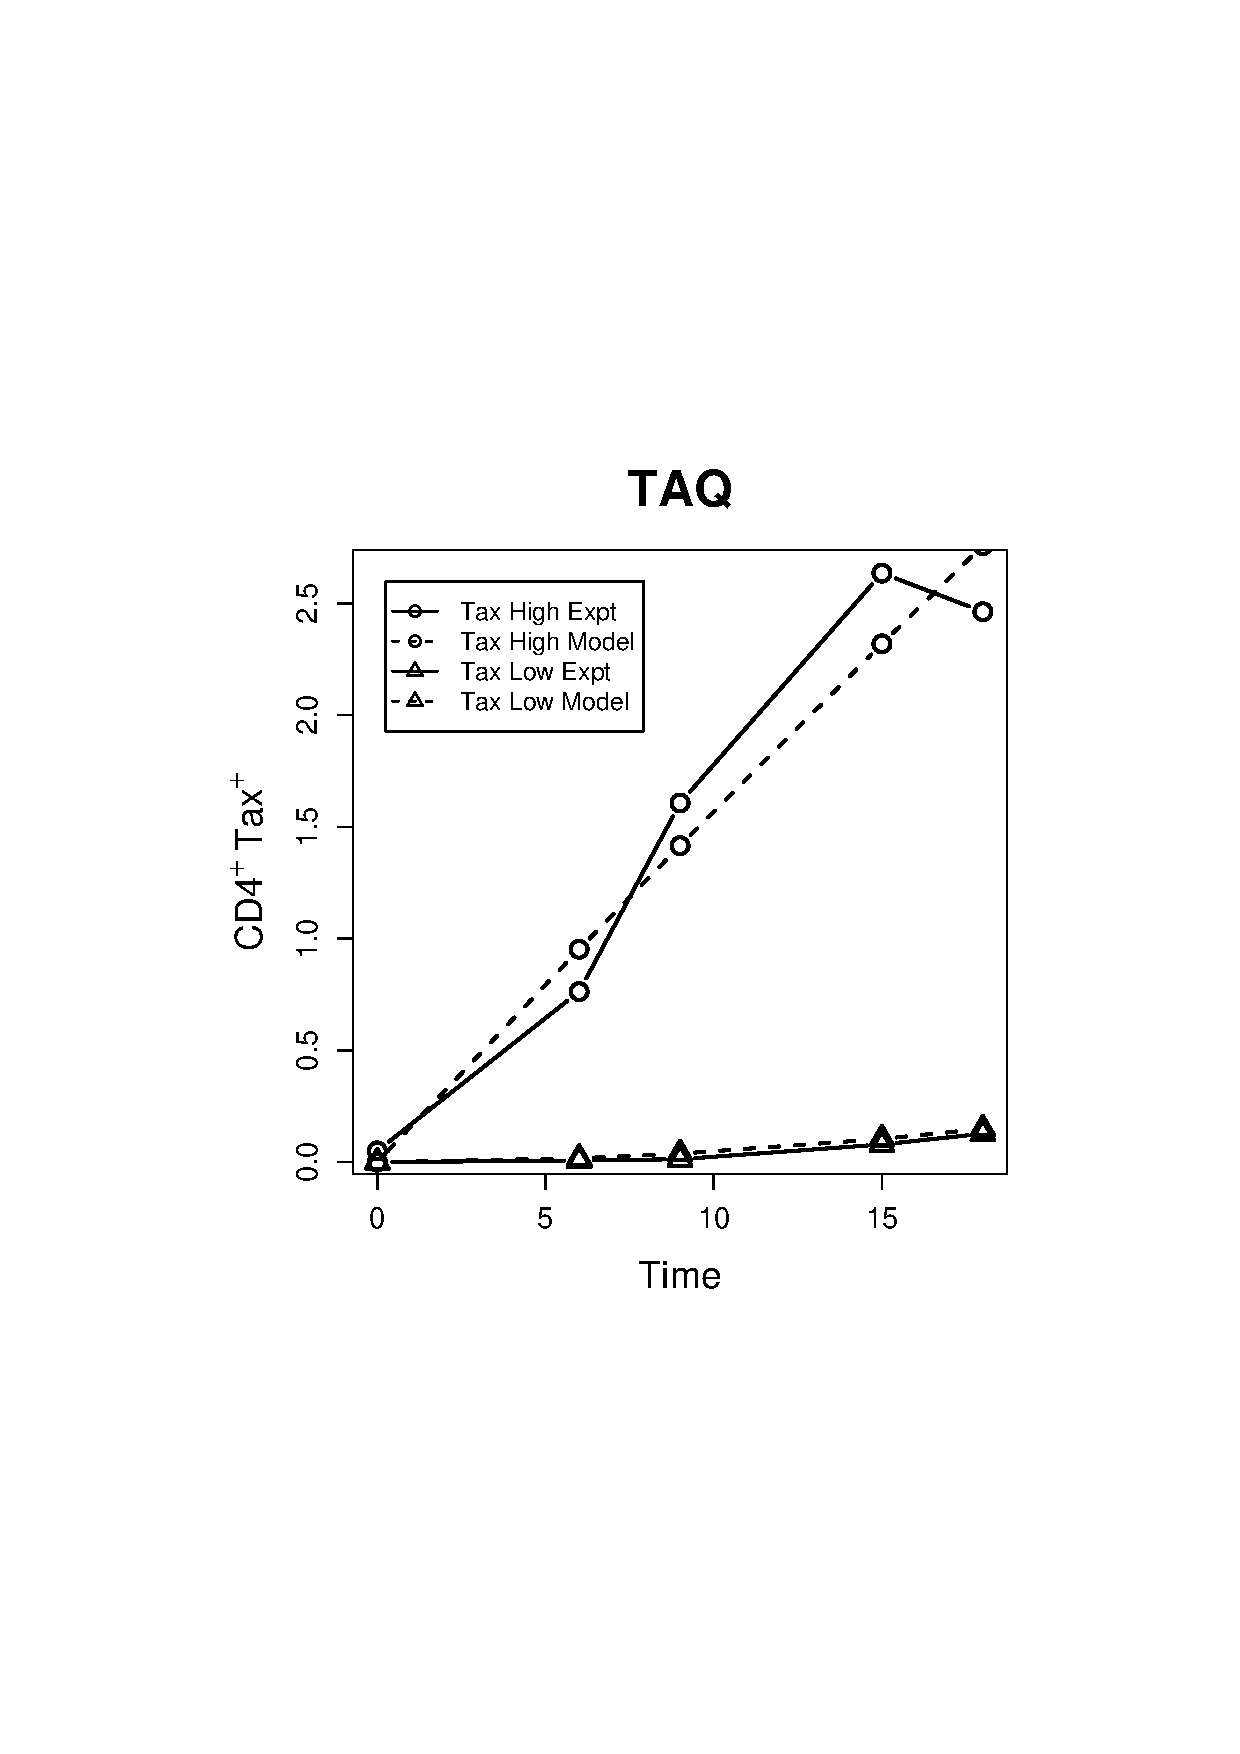
\includegraphics[width=7cm]{./Figures/chapter5/figure_timecourse_taq} \\
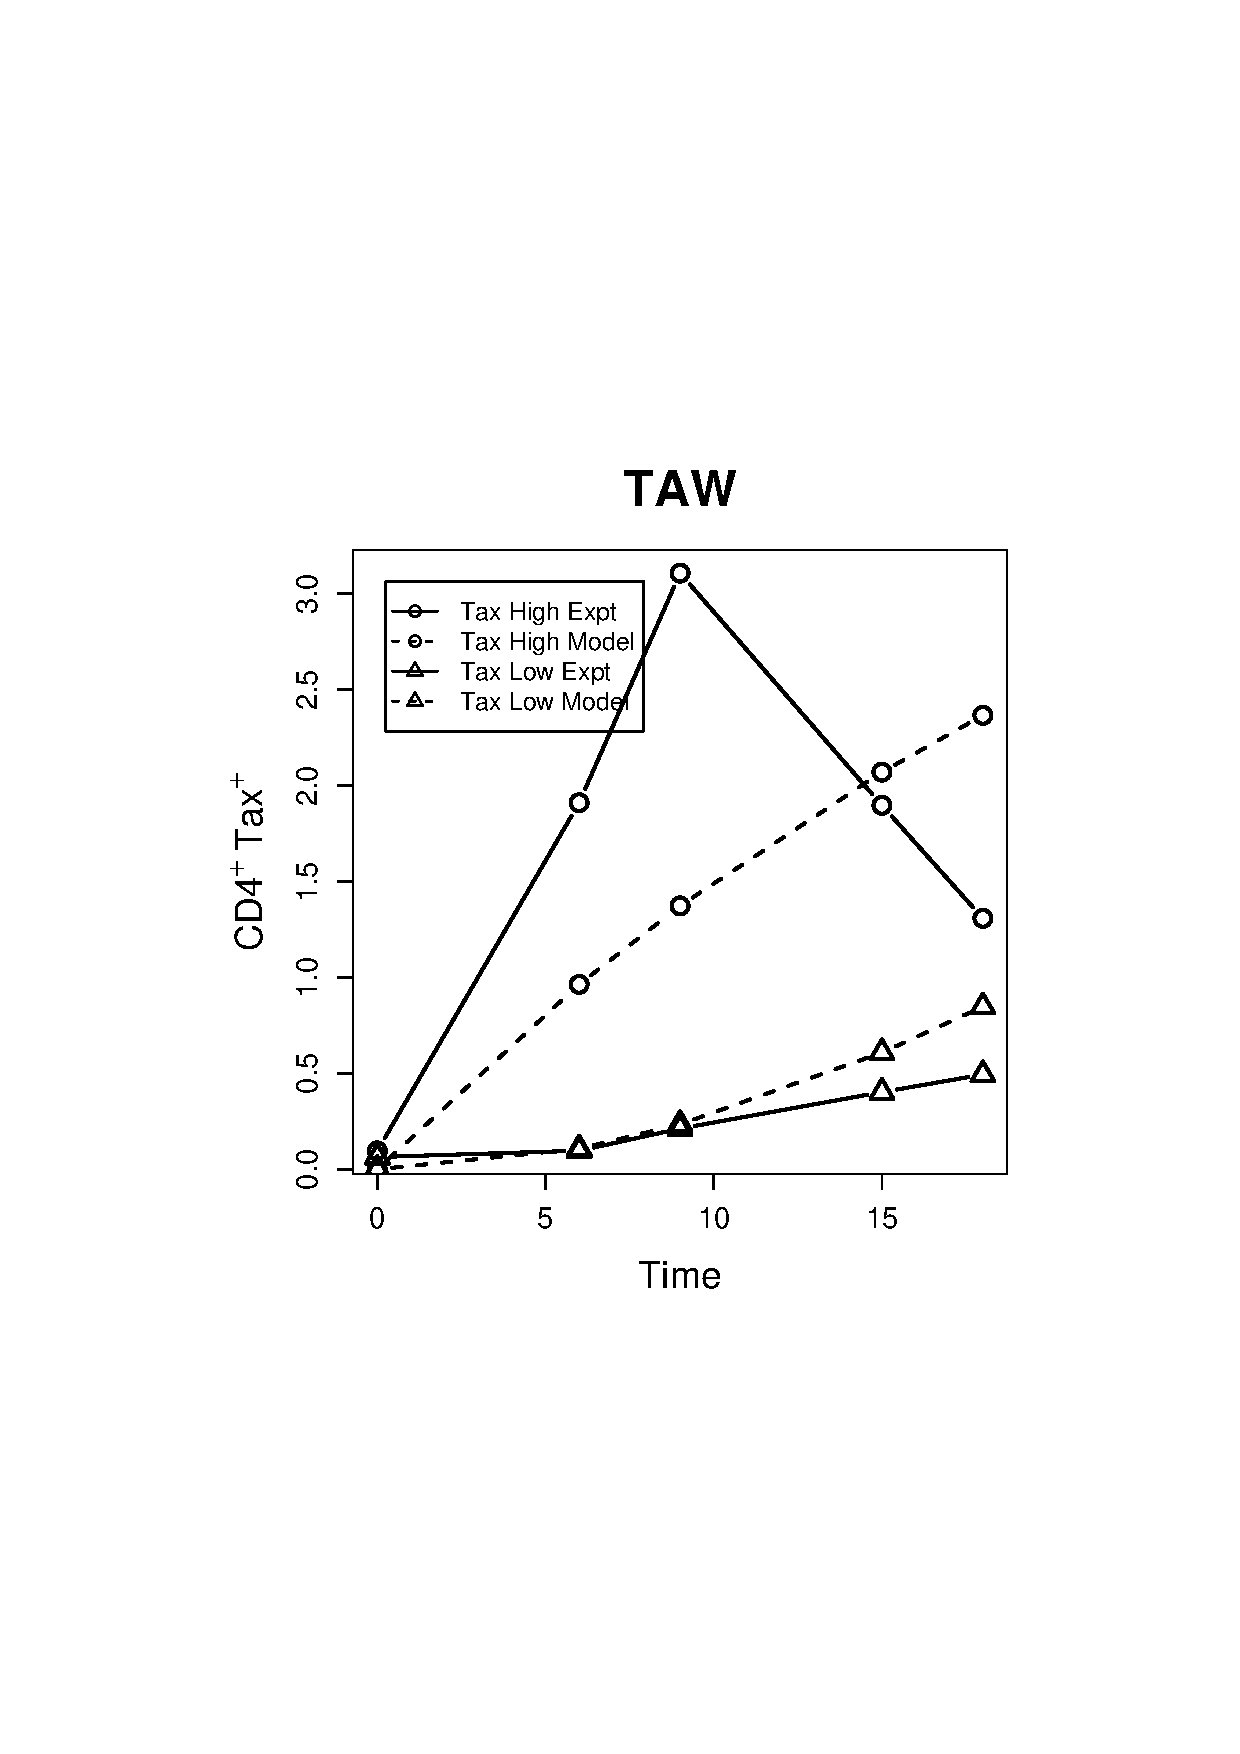
\includegraphics[width=7cm]{./Figures/chapter5/figure_timecourse_taw}%
\hspace{0cm}%
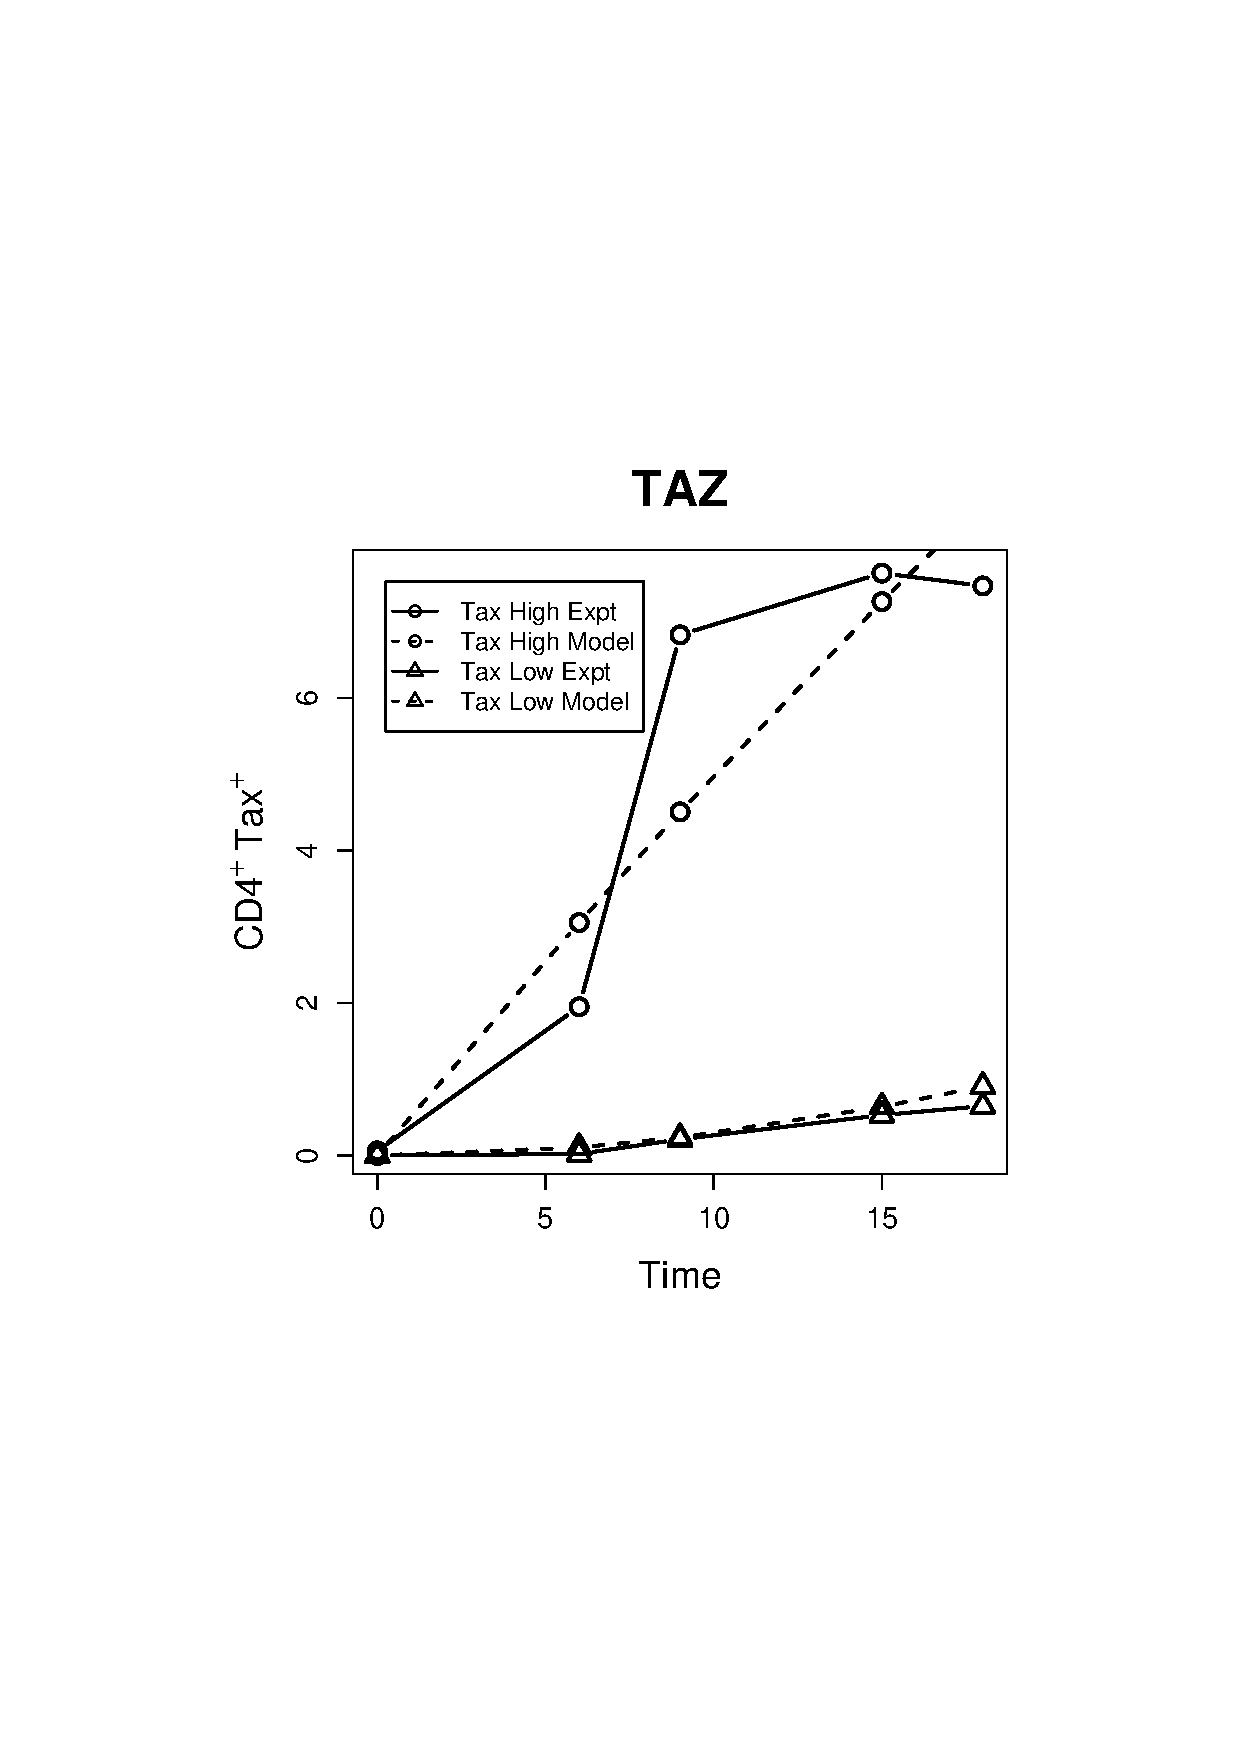
\includegraphics[width=7cm]{./Figures/chapter5/figure_timecourse_taz} \\
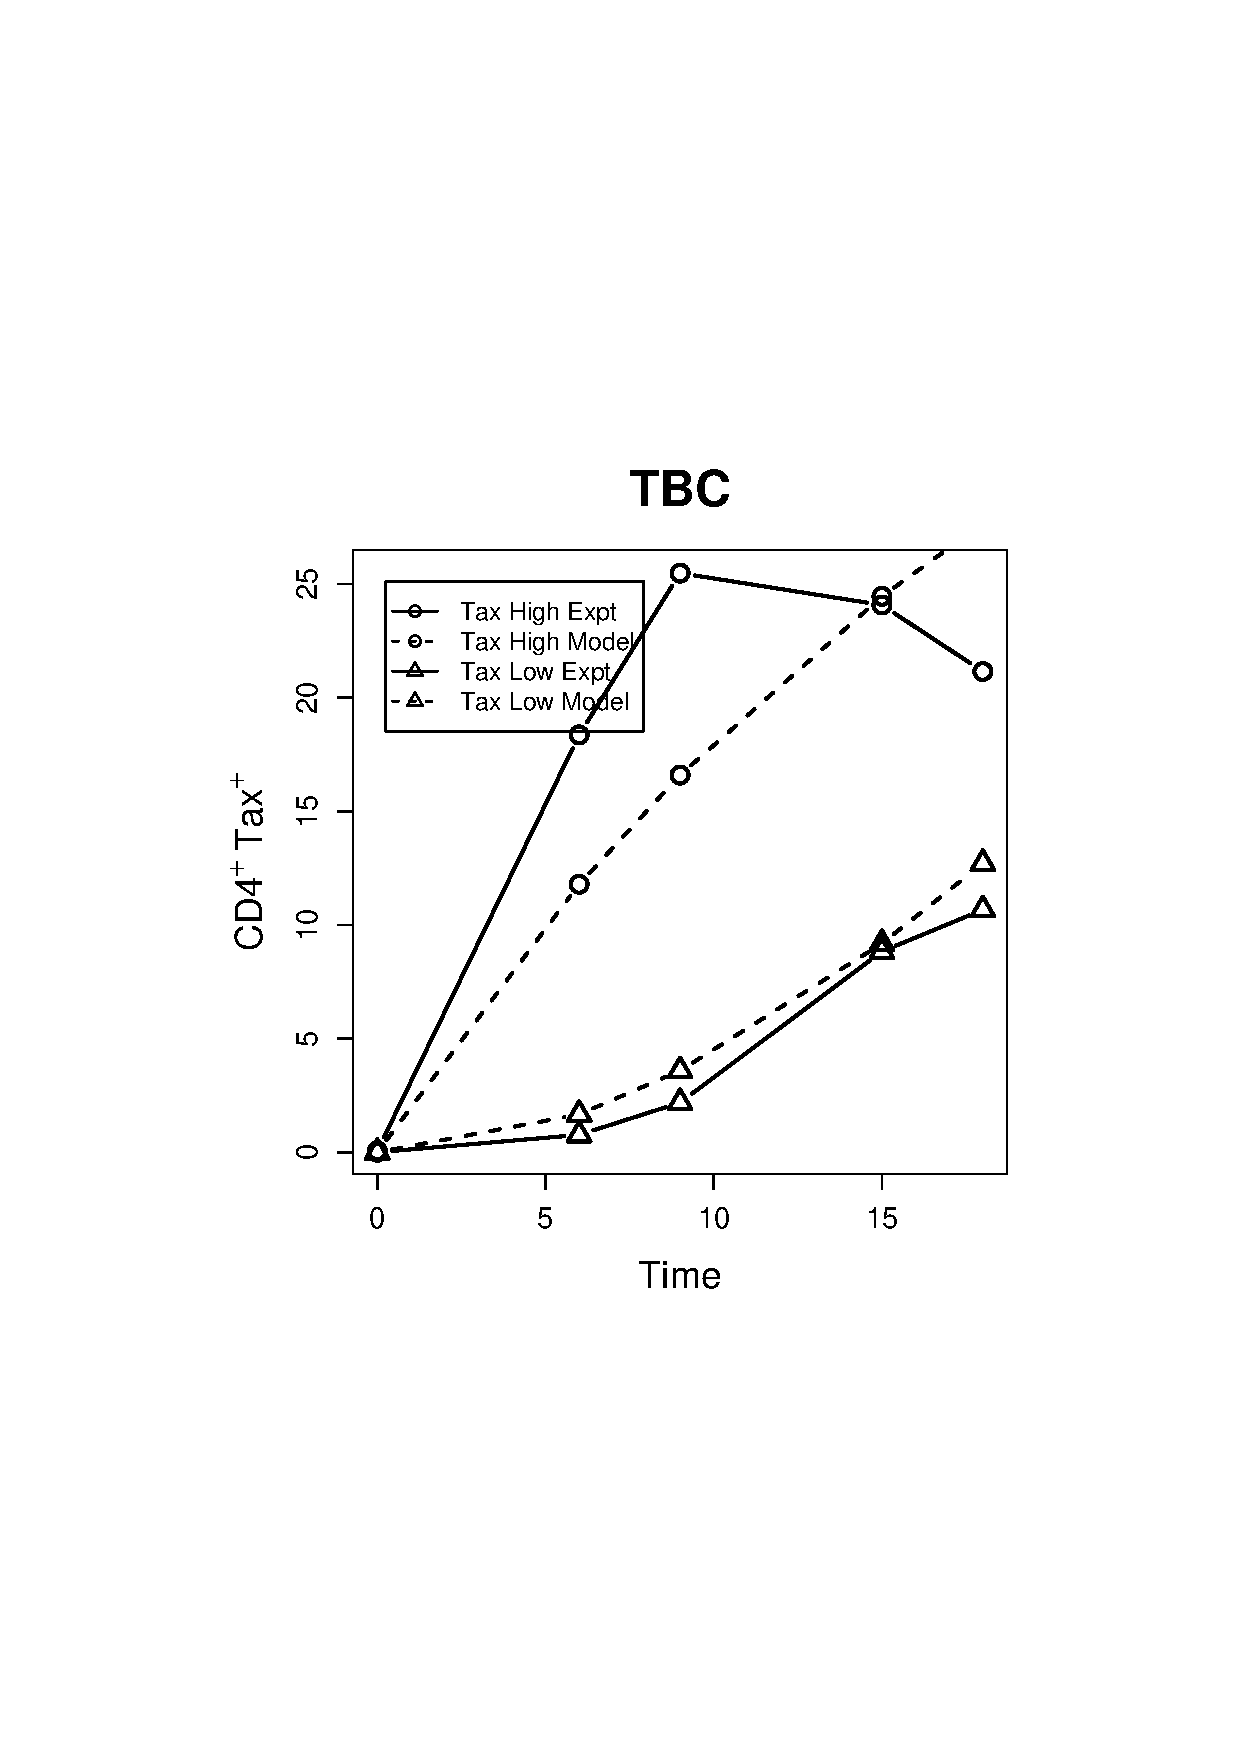
\includegraphics[width=7cm]{./Figures/chapter5/figure_timecourse_tbc}%
\hspace{0cm}%
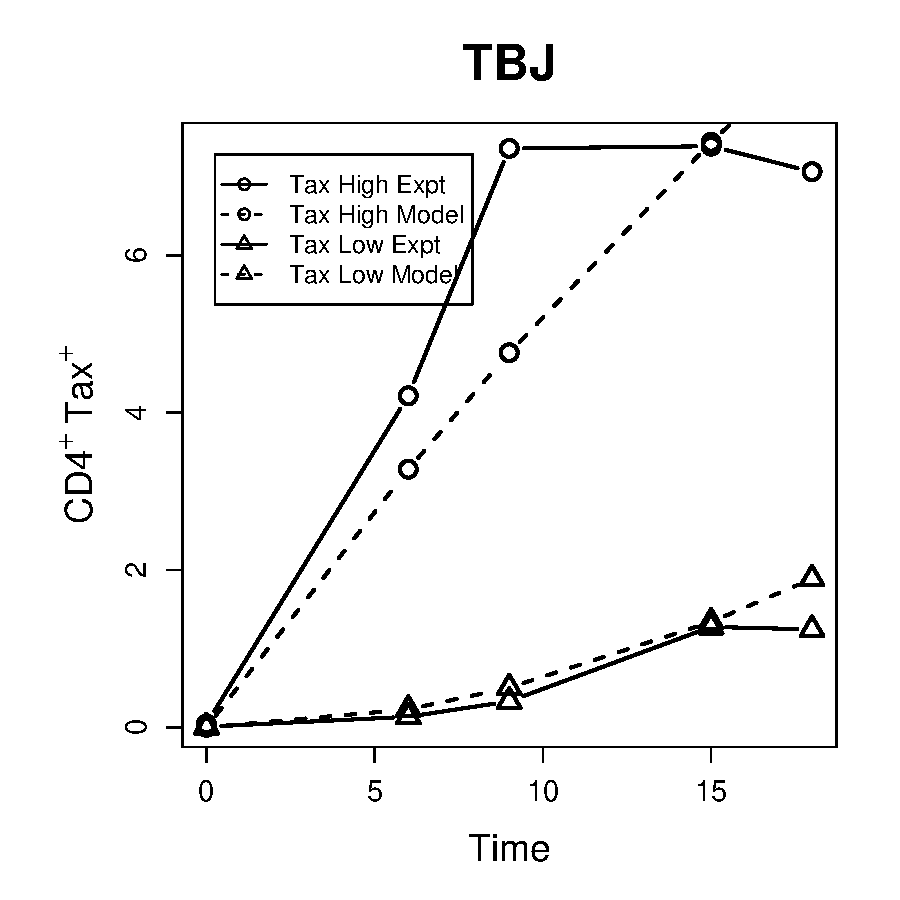
\includegraphics[width=7cm]{./Figures/chapter5/figure_timecourse_tbj} \\
\caption[The Tax expression time course: other patients]{The time course of Tax expression as the proportion of CD4$^+$ lymphocytes that were Tax\superscript{high} or Tax\superscript{low}. The supplementary data from \fref{chapter5/figureTimeCourse}.}
\label{appendixb/figureTimecourse}
\end{figure}

\begin{figure}[htp]
\flushleft
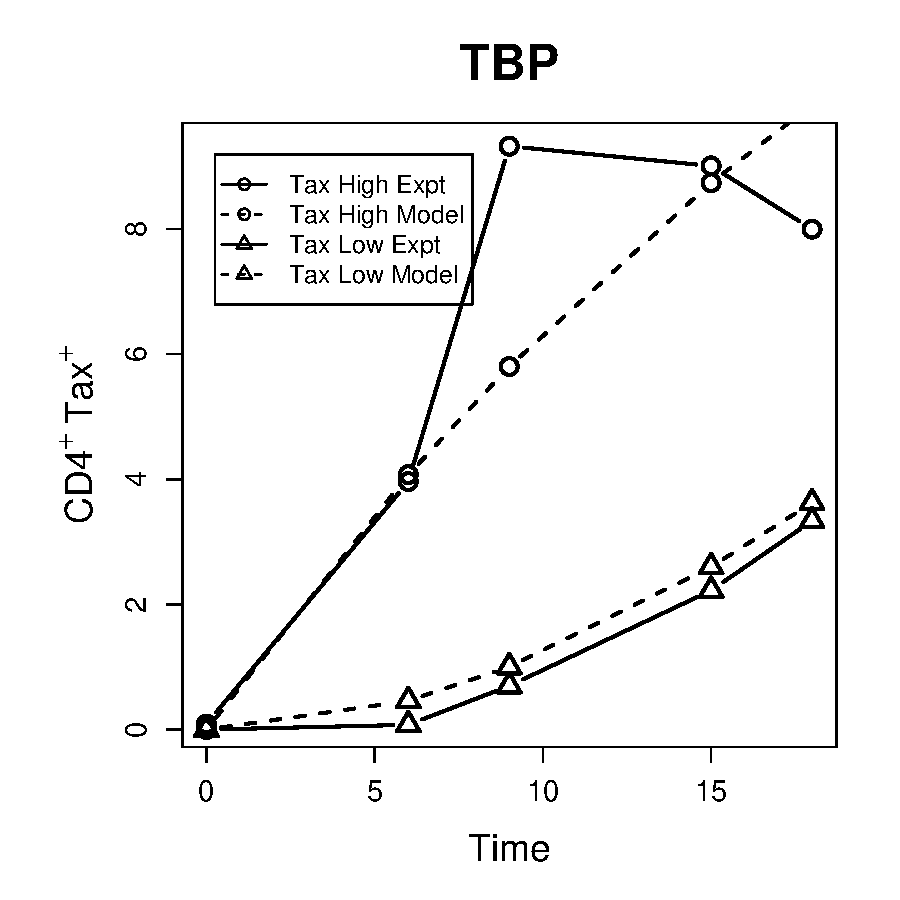
\includegraphics[width=7cm]{./Figures/chapter5/figure_timecourse_tbp}%
\hspace{0cm}%
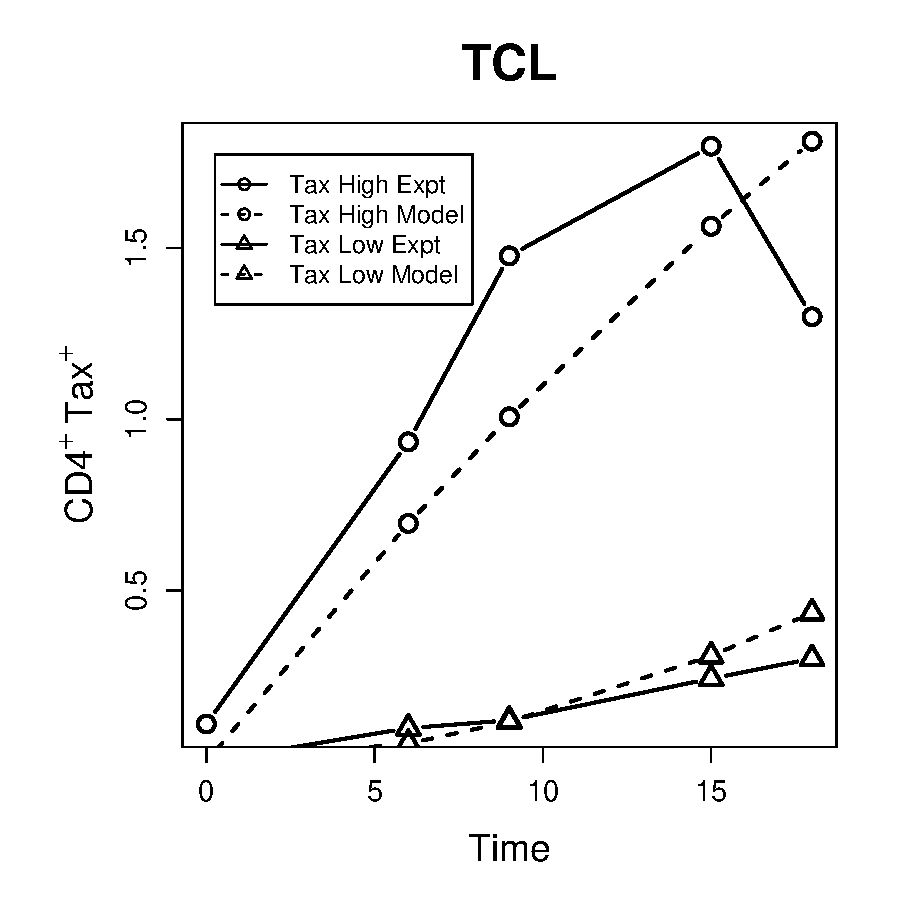
\includegraphics[width=7cm]{./Figures/chapter5/figure_timecourse_tcl} \\
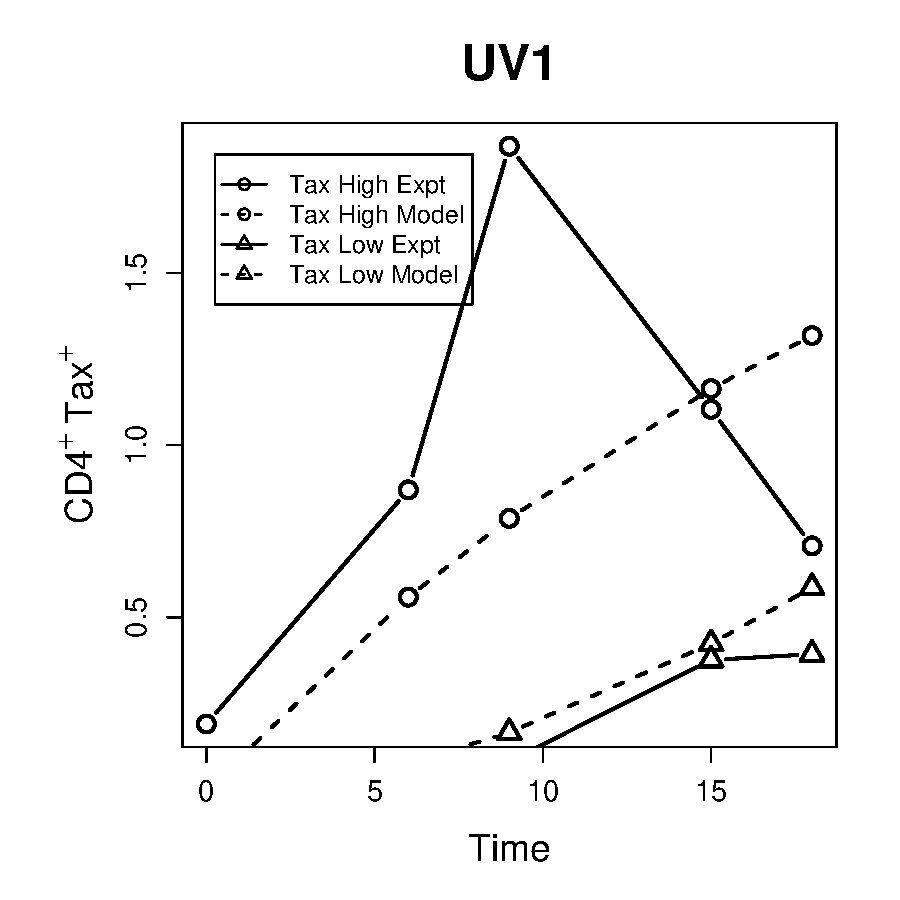
\includegraphics[width=7cm]{./Figures/chapter5/figure_timecourse_uv1}%
\contcaption{Continued}
\end{figure}

%%%%%%%%%%%%%%%%%%%%%%%%%%%%%%%%%%%%%%%%%%%%%%%%%%%%%%%%%%%%%%%%%%%%%%%%%%%%%%%%%%%%%%%%%%%%%%%%%%%%

\begin{figure}[htp]
\centering
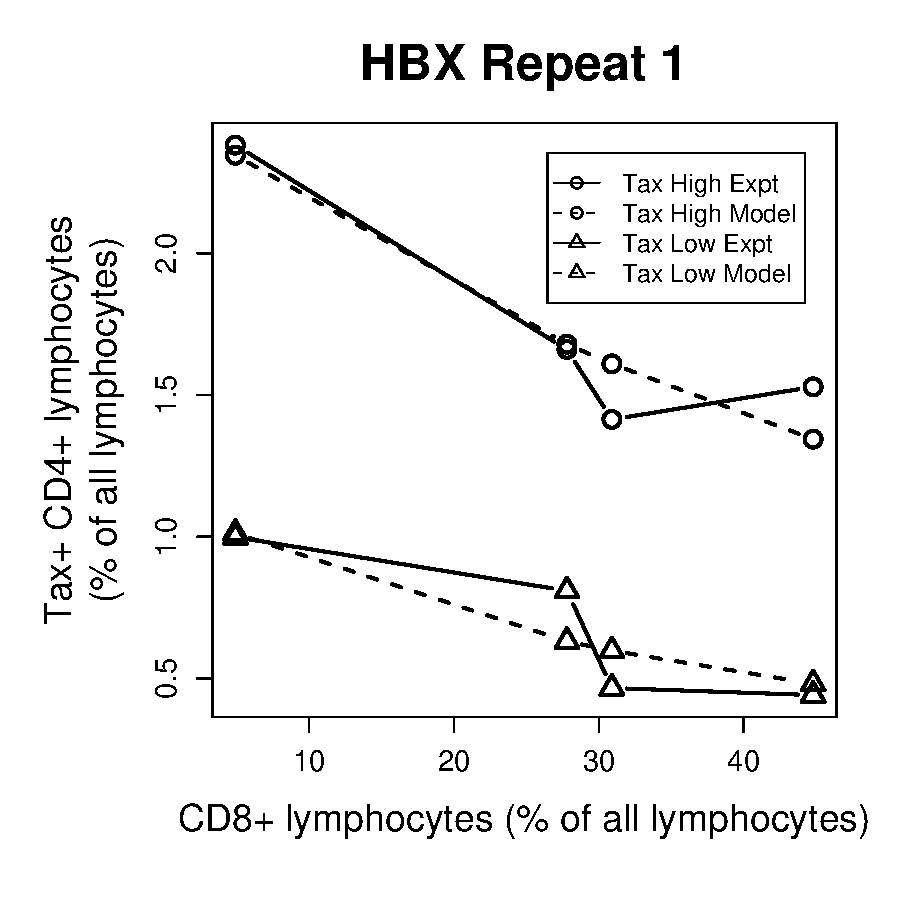
\includegraphics[width=7cm]{./Figures/chapter5/figure_lysis_hbx_rep_1}%
\hspace{0cm}%
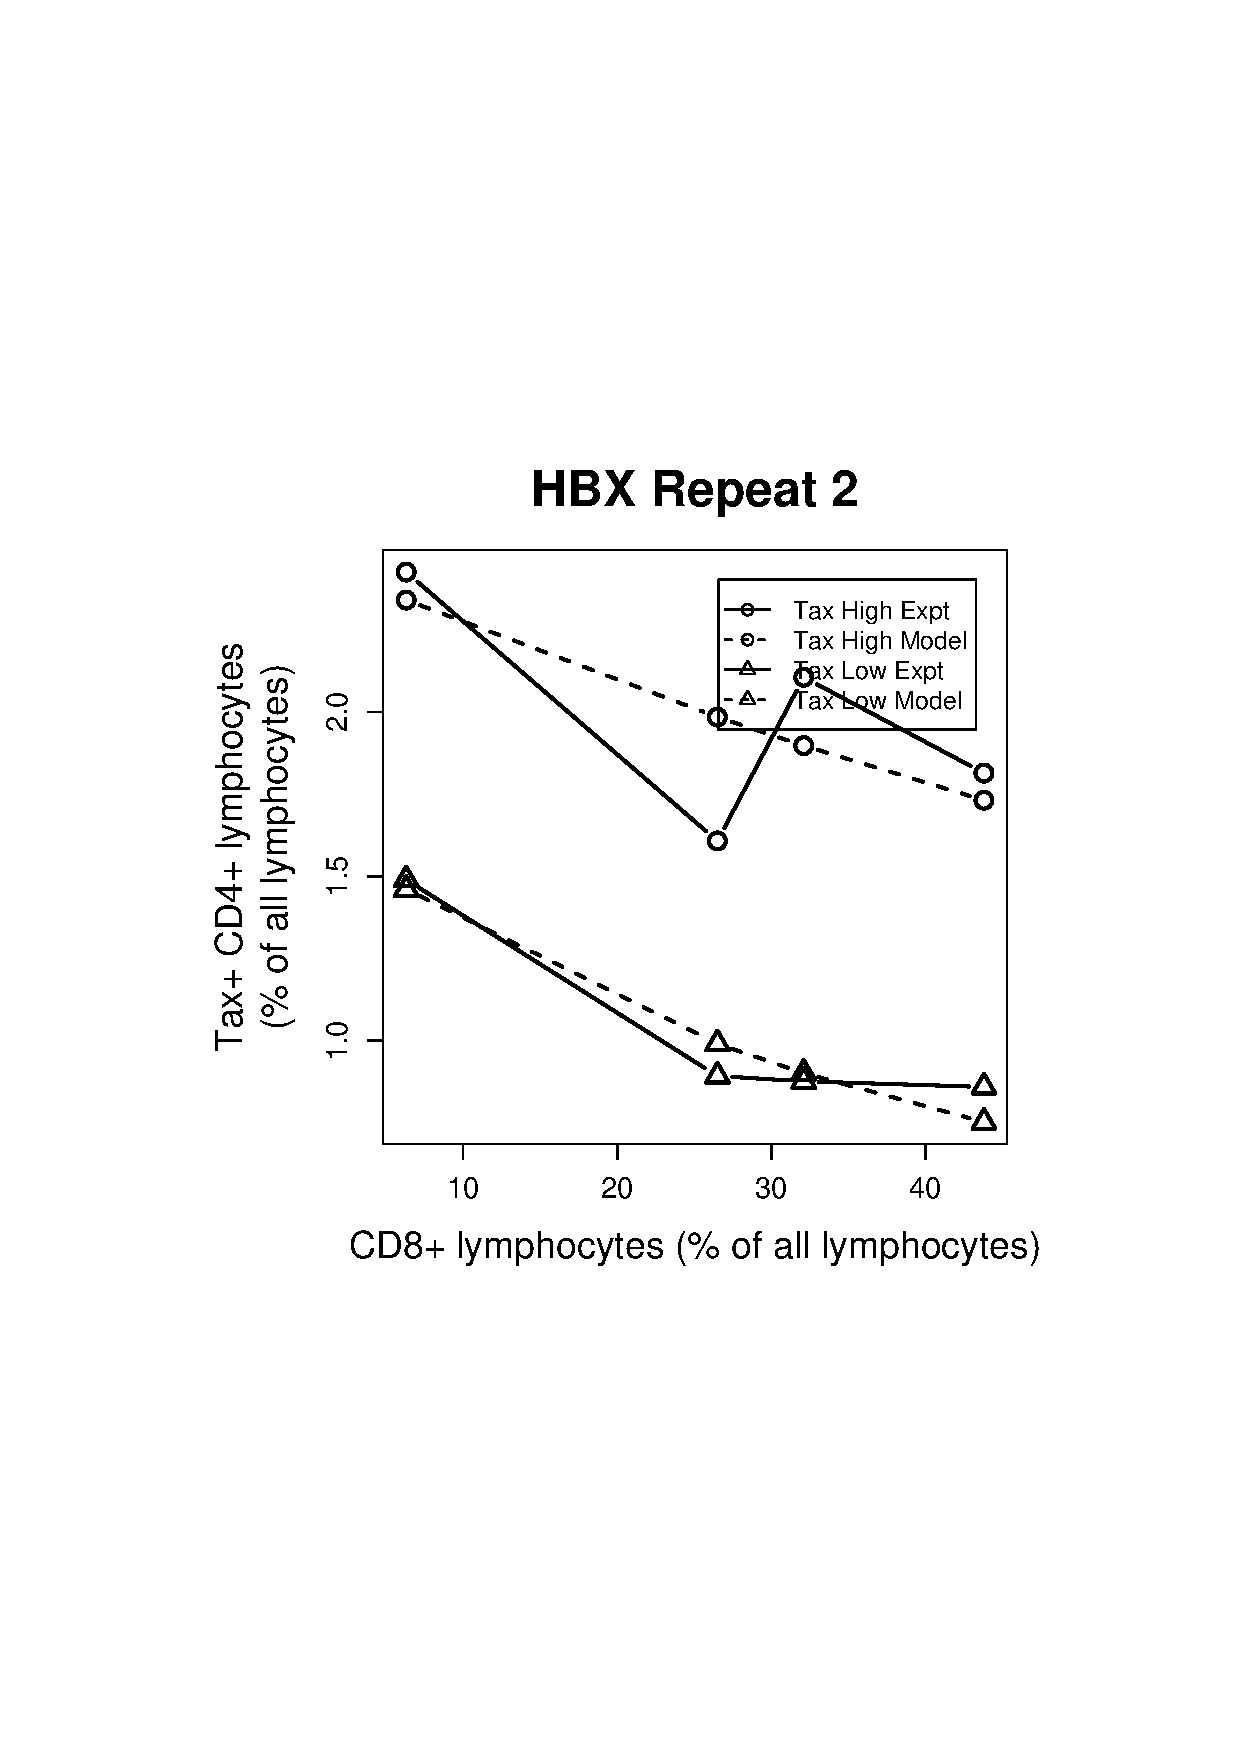
\includegraphics[width=7cm]{./Figures/chapter5/figure_lysis_hbx_rep_2} \\
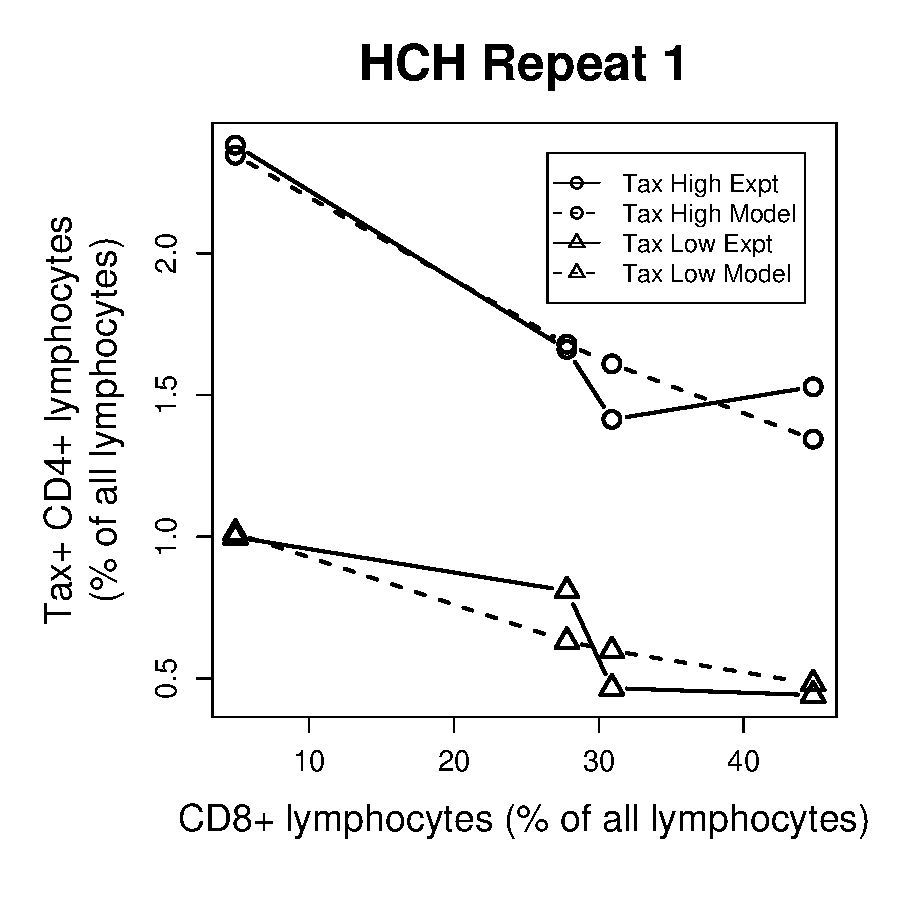
\includegraphics[width=7cm]{./Figures/chapter5/figure_lysis_hch_rep_1}%
\hspace{0cm}%
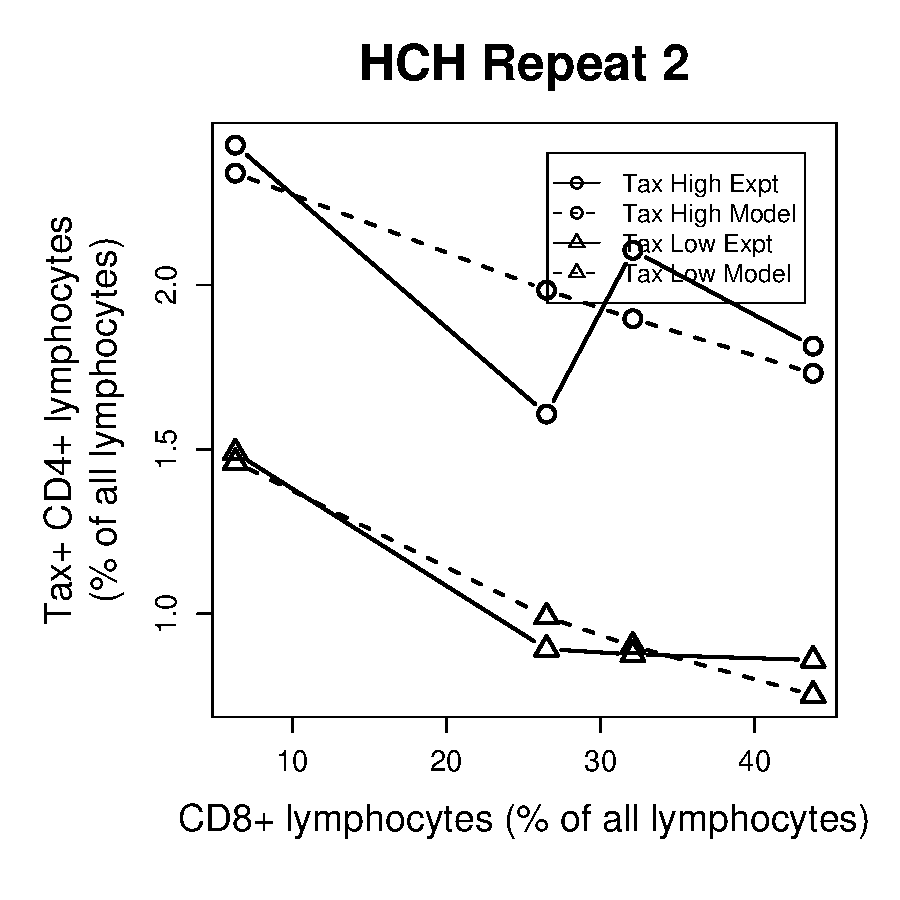
\includegraphics[width=7cm]{./Figures/chapter5/figure_lysis_hch_rep_2} \\
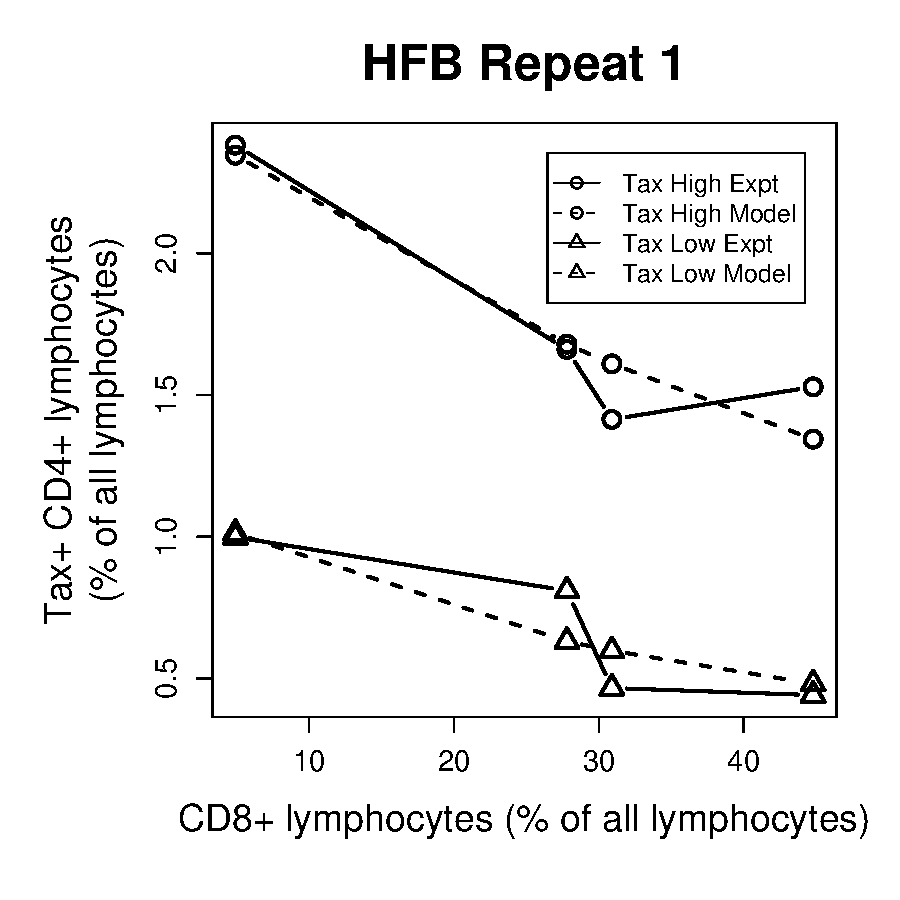
\includegraphics[width=7cm]{./Figures/chapter5/figure_lysis_hfb_rep_1}%
\hspace{0cm}%
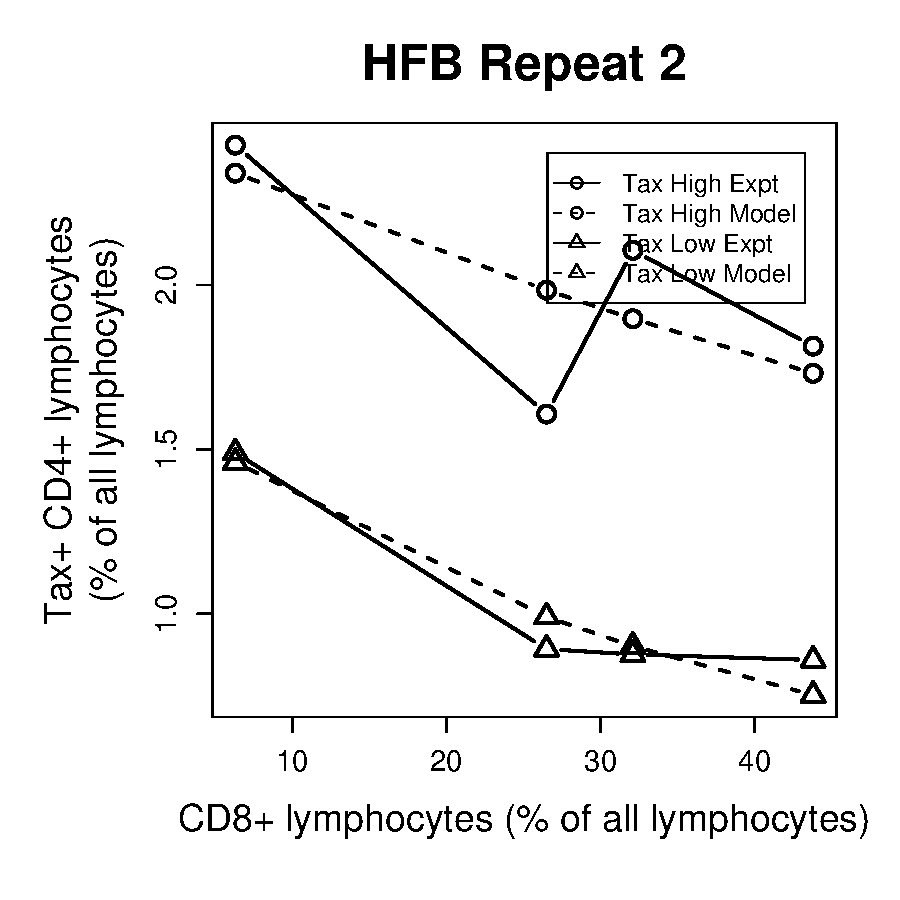
\includegraphics[width=7cm]{./Figures/chapter5/figure_lysis_hfb_rep_2} \\
\caption[CD8$^+$ antiviral efficacy assay: other patients]{The proportion of CD4$^+$ lymphocytes that were Tax\superscript{high} and Tax\superscript{low} following 18 h co-culture with different proportions of CD8$^+$ lymphocytes. The supplementary data from \fref{chapter5/figureLysisAssay}.}
\label{appendixb/figureLysisHighLow}
\end{figure}

\begin{figure}[htp]
\centering
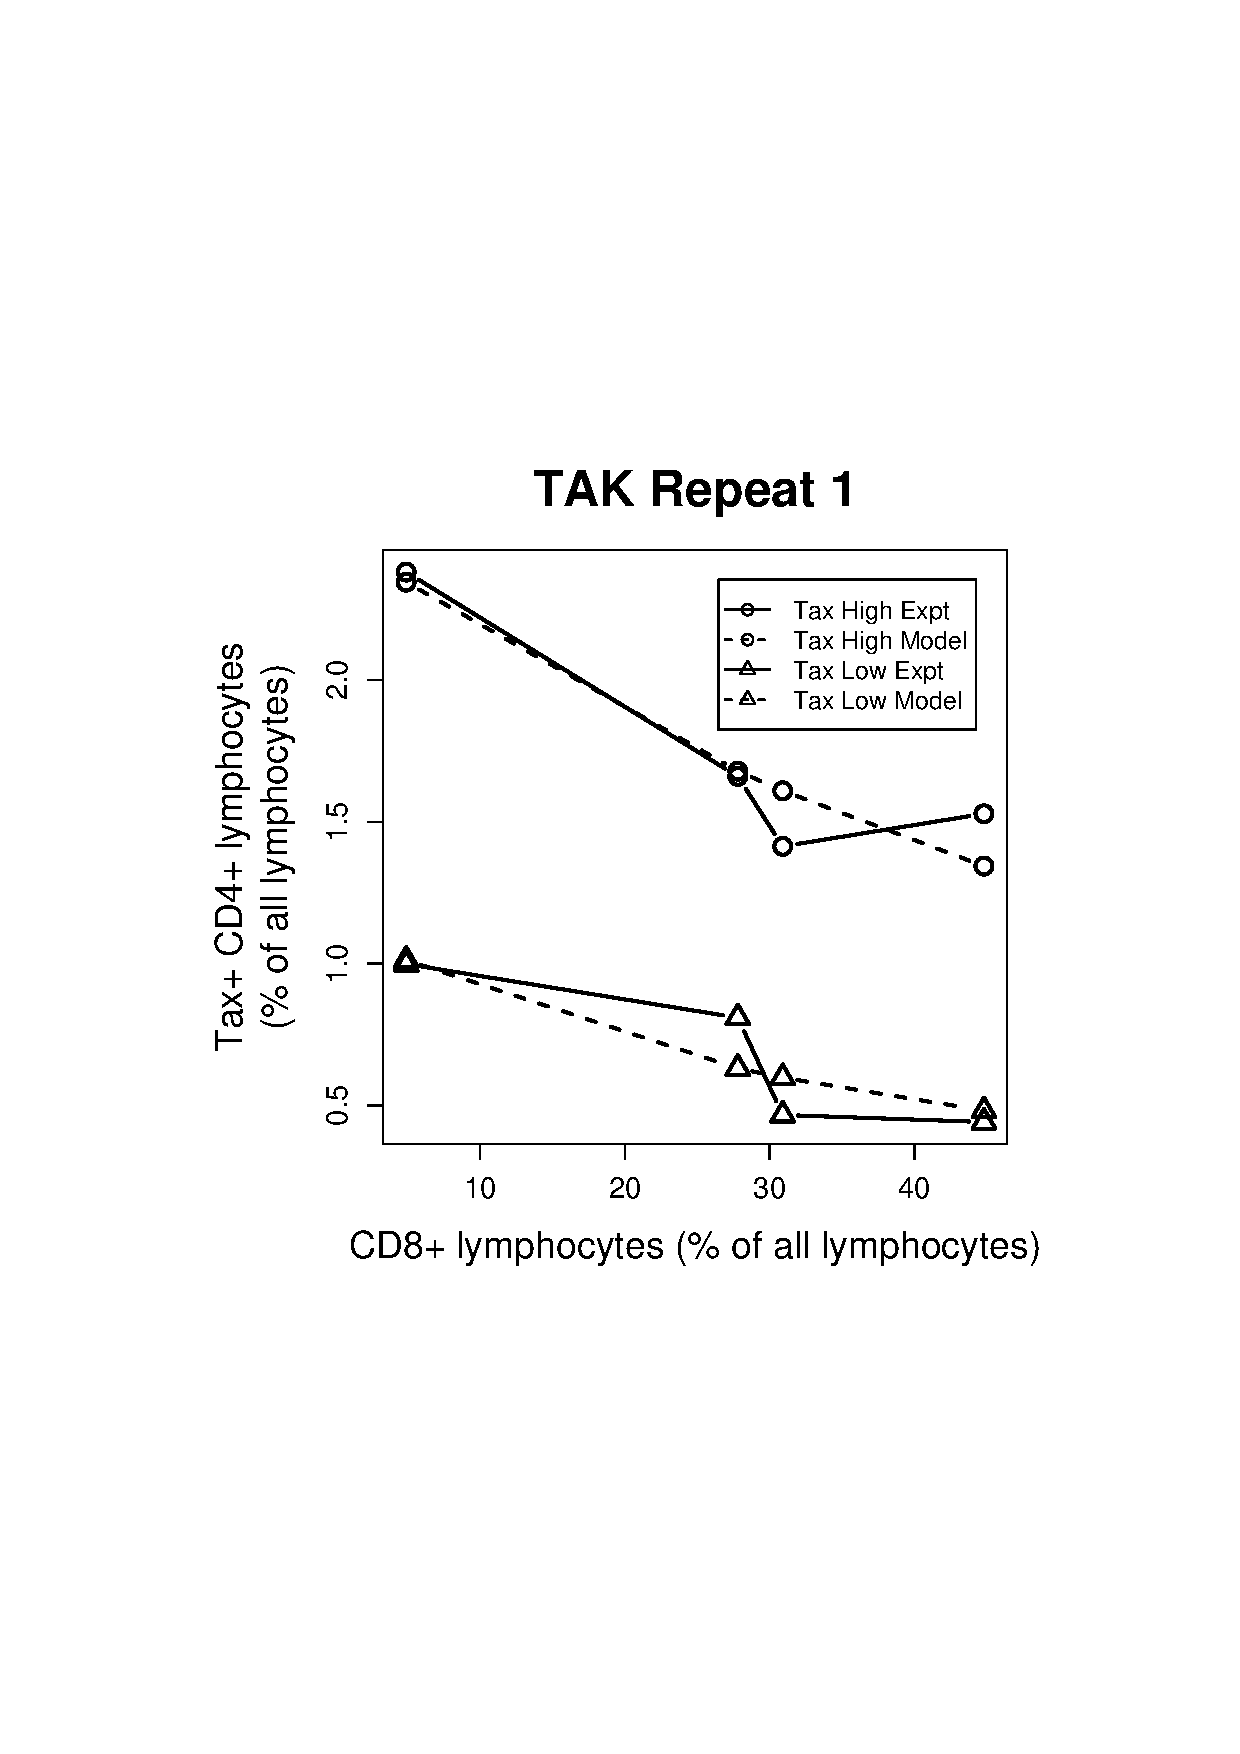
\includegraphics[width=7cm]{./Figures/chapter5/figure_lysis_tak_rep_1}%
\hspace{0cm}%
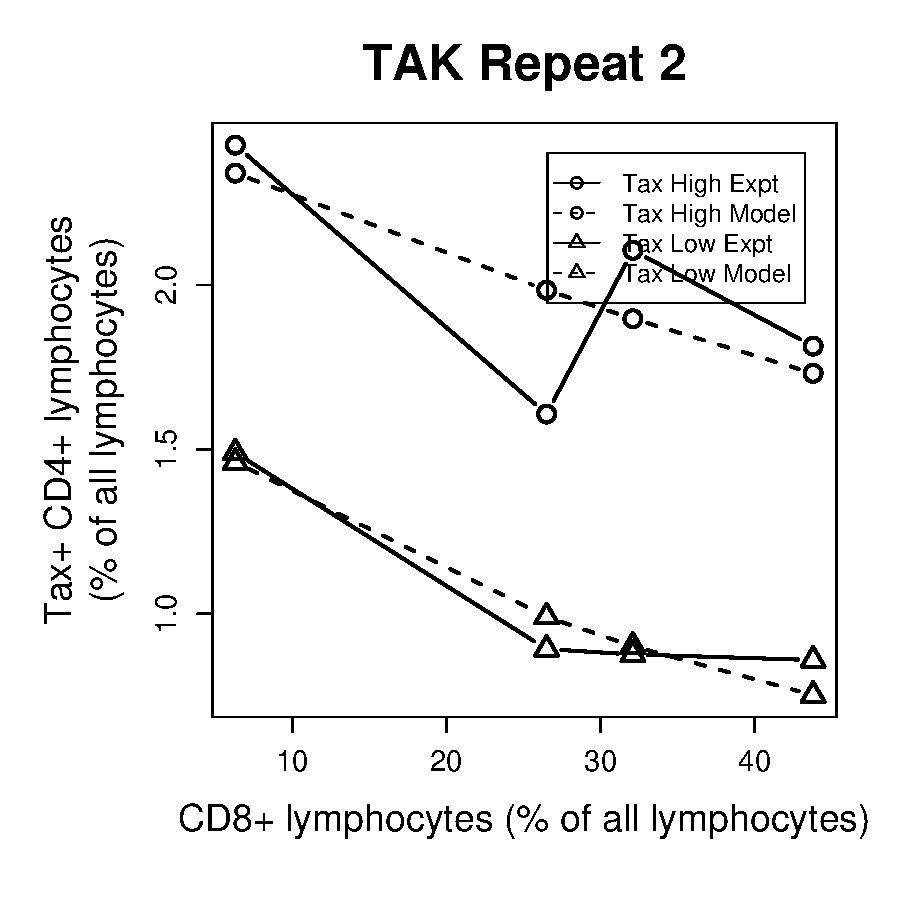
\includegraphics[width=7cm]{./Figures/chapter5/figure_lysis_tak_rep_2} \\
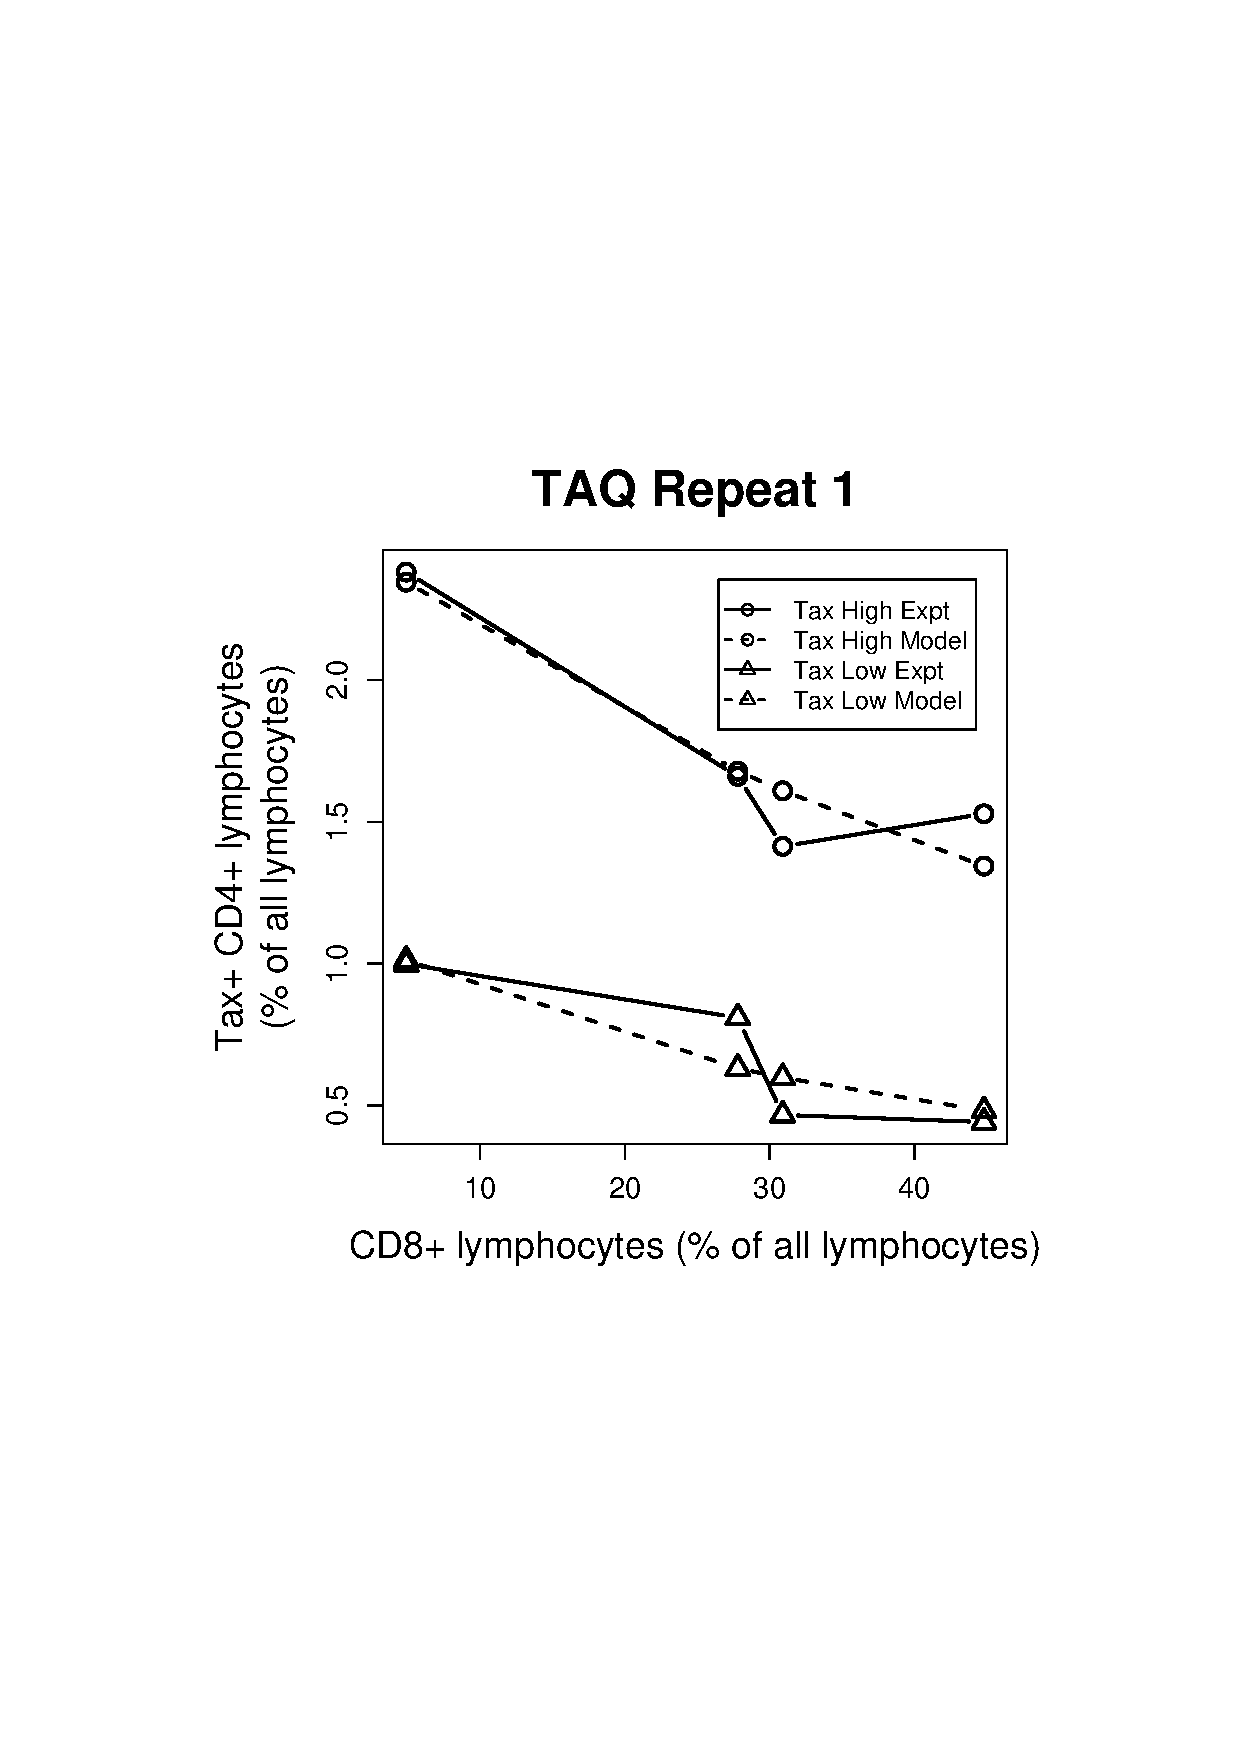
\includegraphics[width=7cm]{./Figures/chapter5/figure_lysis_taq_rep_1}%
\hspace{0cm}%
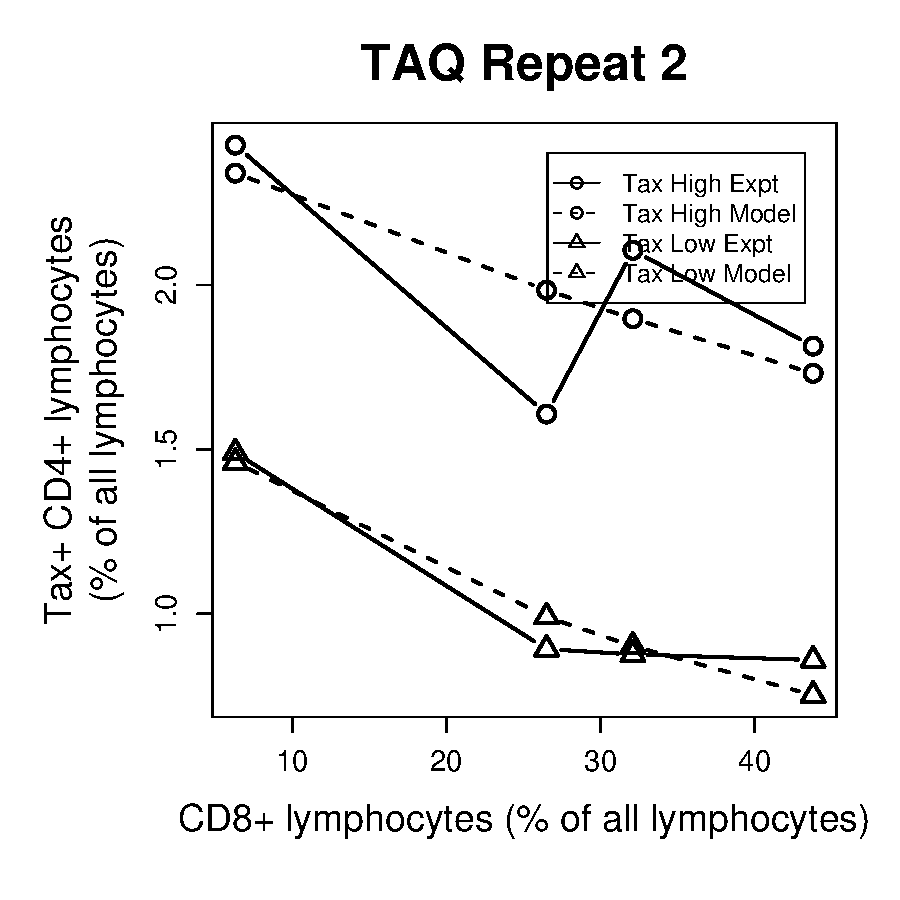
\includegraphics[width=7cm]{./Figures/chapter5/figure_lysis_taq_rep_2} \\
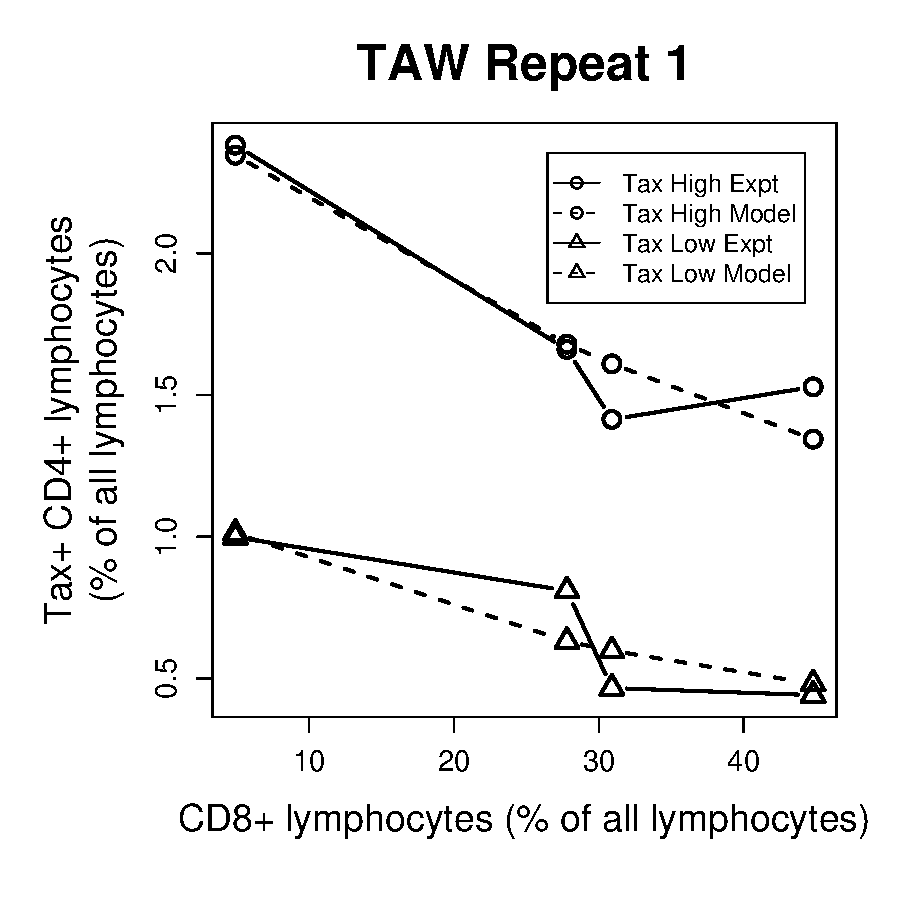
\includegraphics[width=7cm]{./Figures/chapter5/figure_lysis_taw_rep_1}%
\hspace{0cm}%
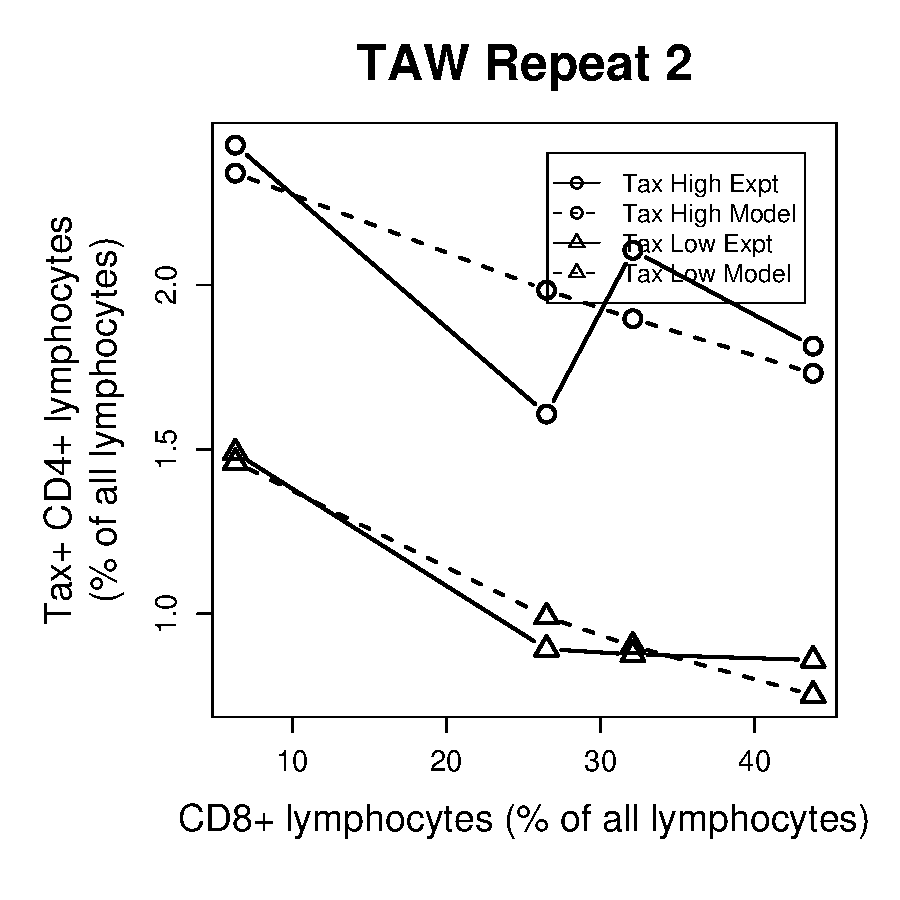
\includegraphics[width=7cm]{./Figures/chapter5/figure_lysis_taw_rep_2} \\
\contcaption{Continued}
\end{figure}

\begin{figure}[htp]
\centering
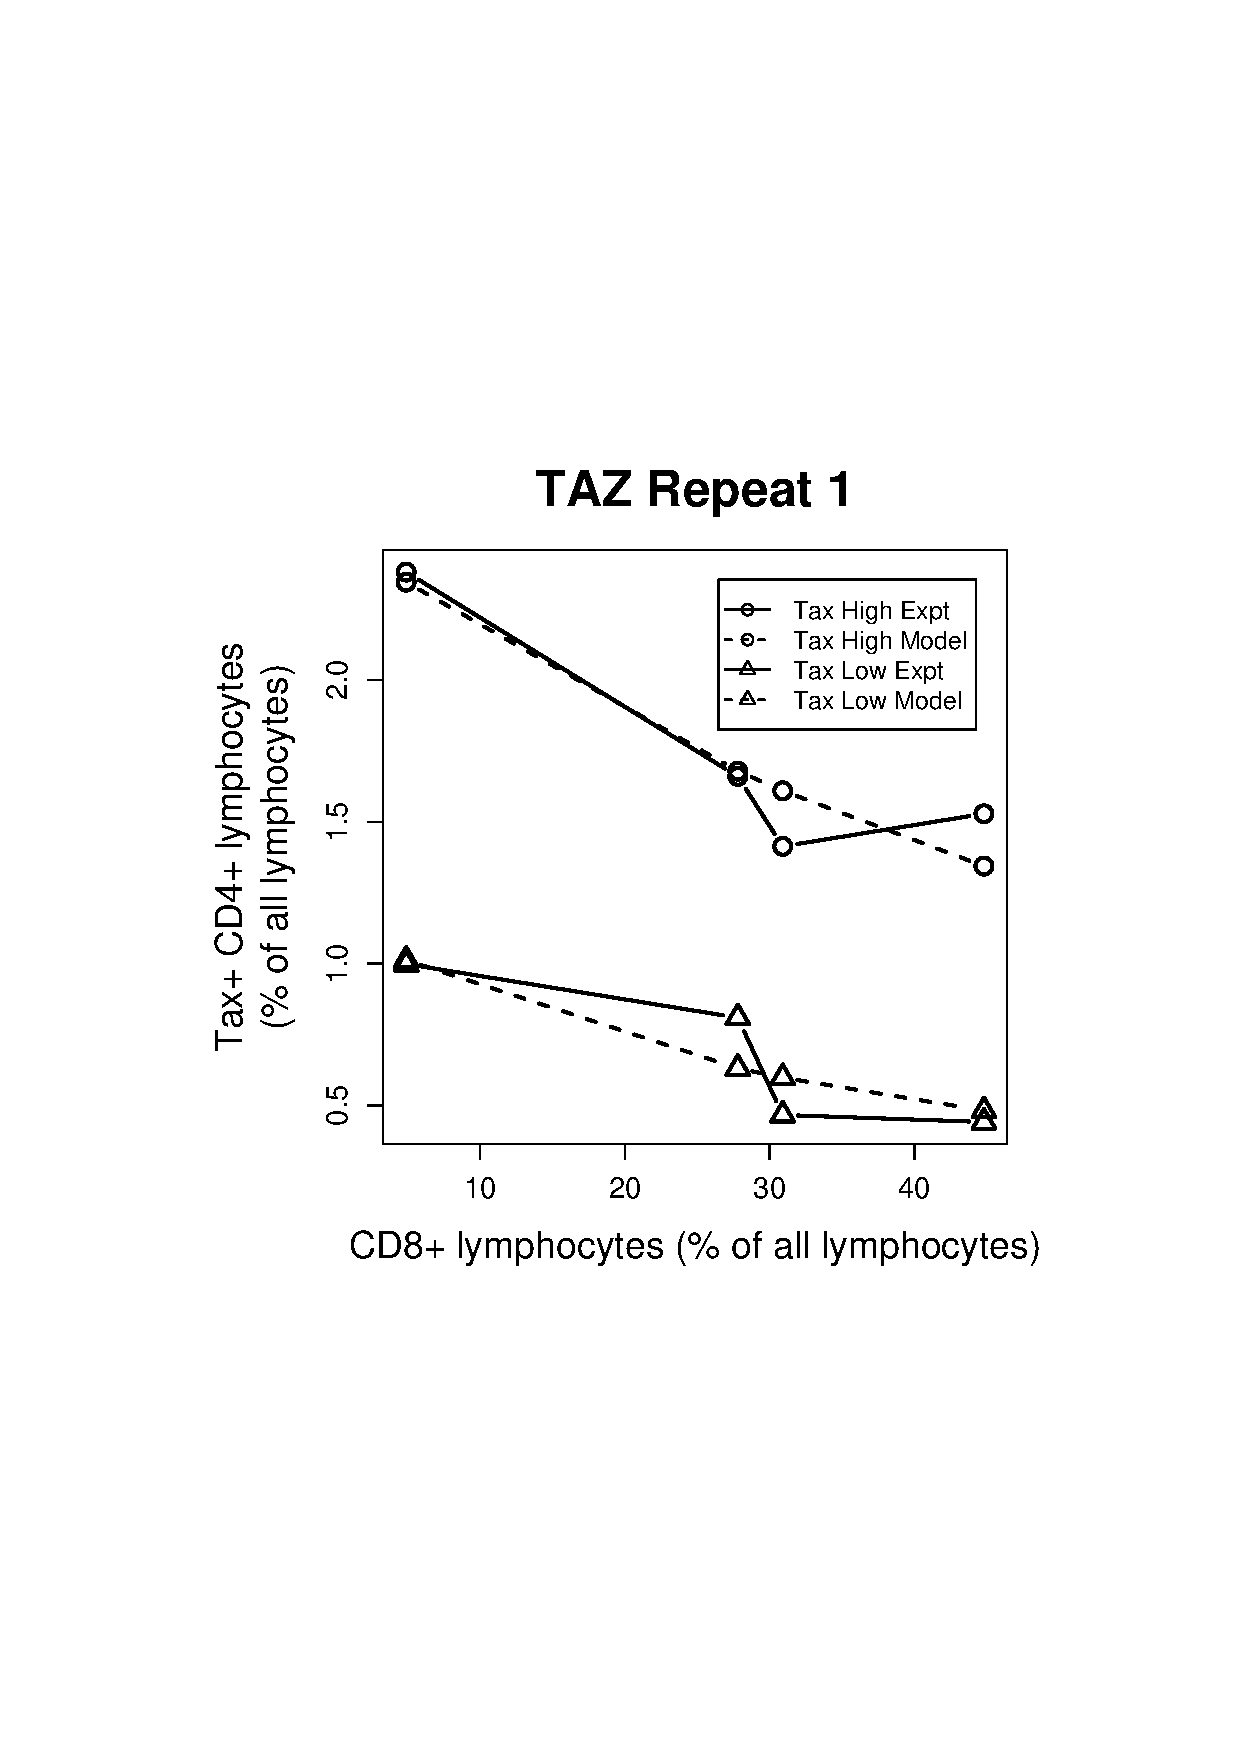
\includegraphics[width=7cm]{./Figures/chapter5/figure_lysis_taz_rep_1}%
\hspace{0cm}%
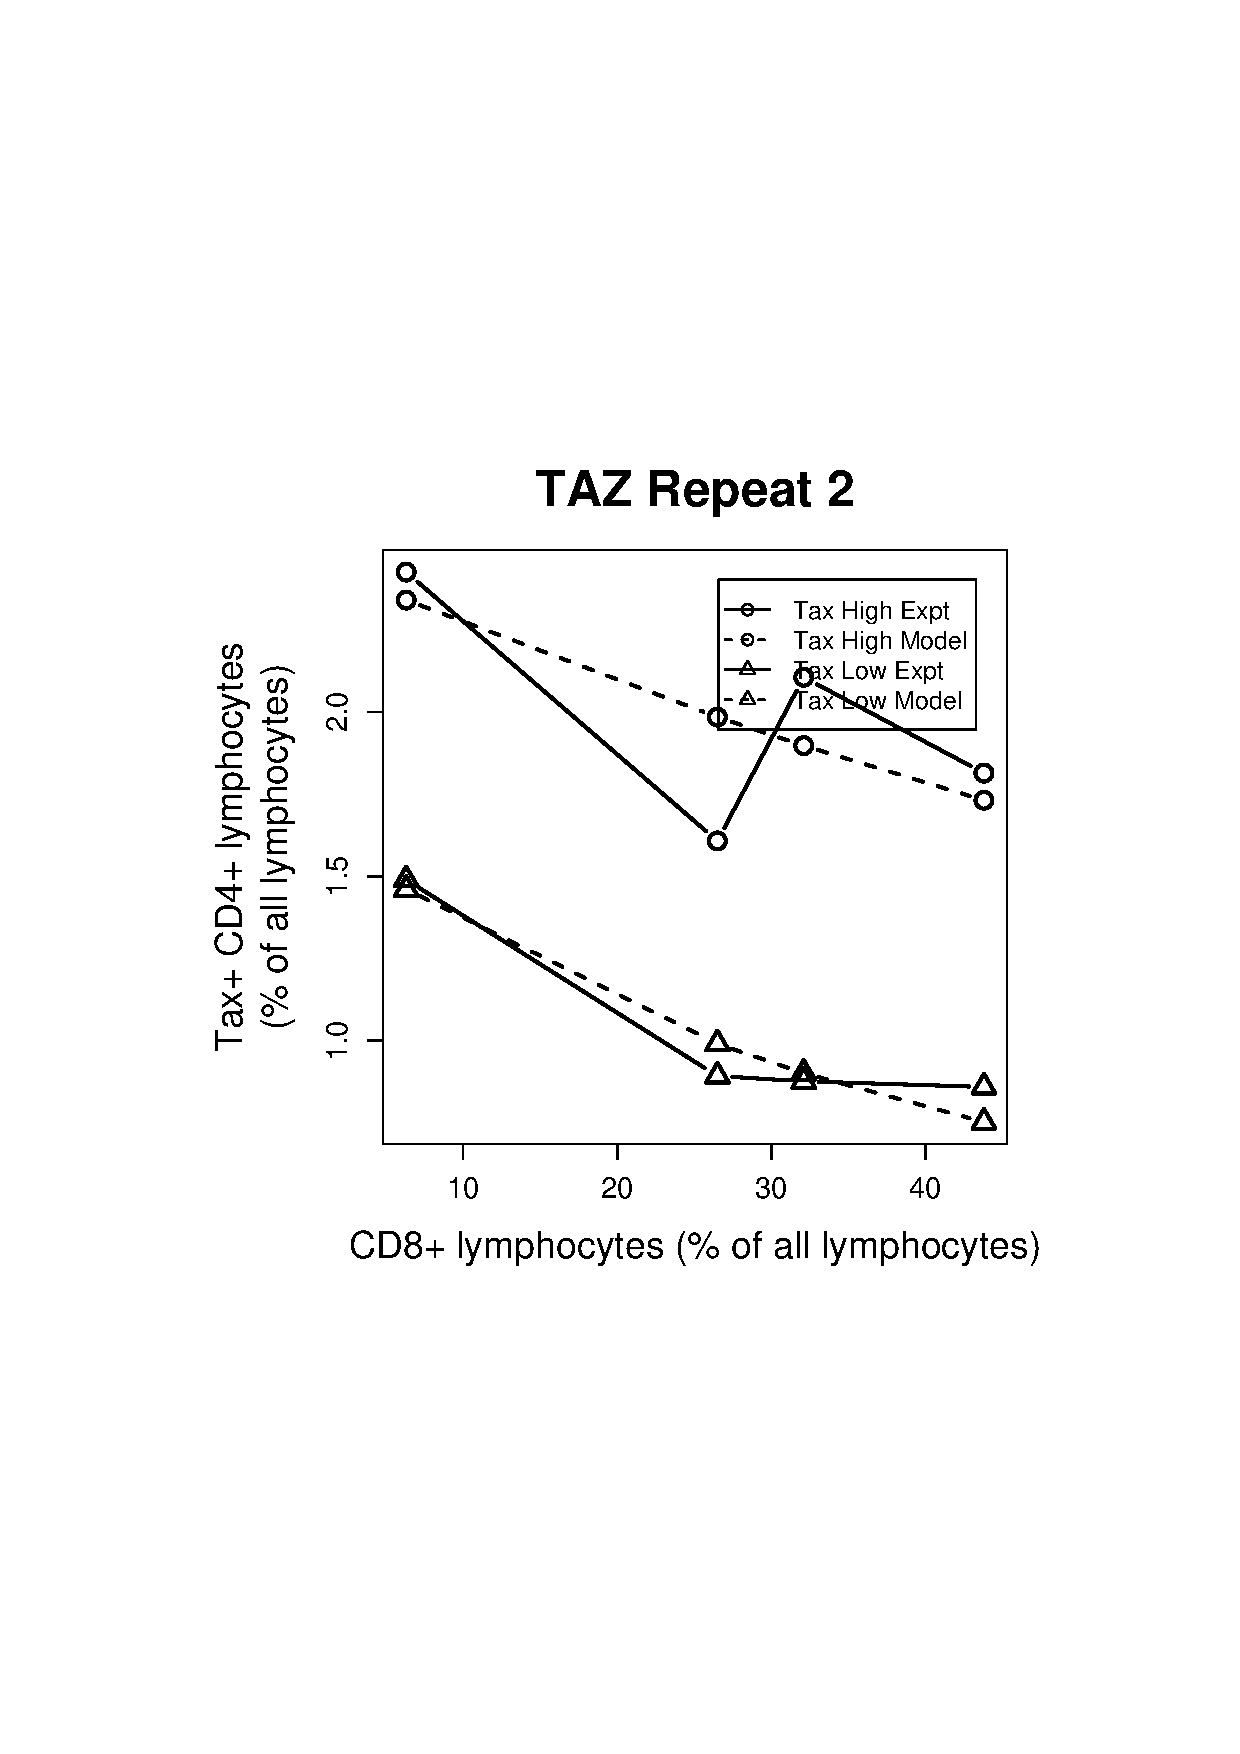
\includegraphics[width=7cm]{./Figures/chapter5/figure_lysis_taz_rep_2} \\
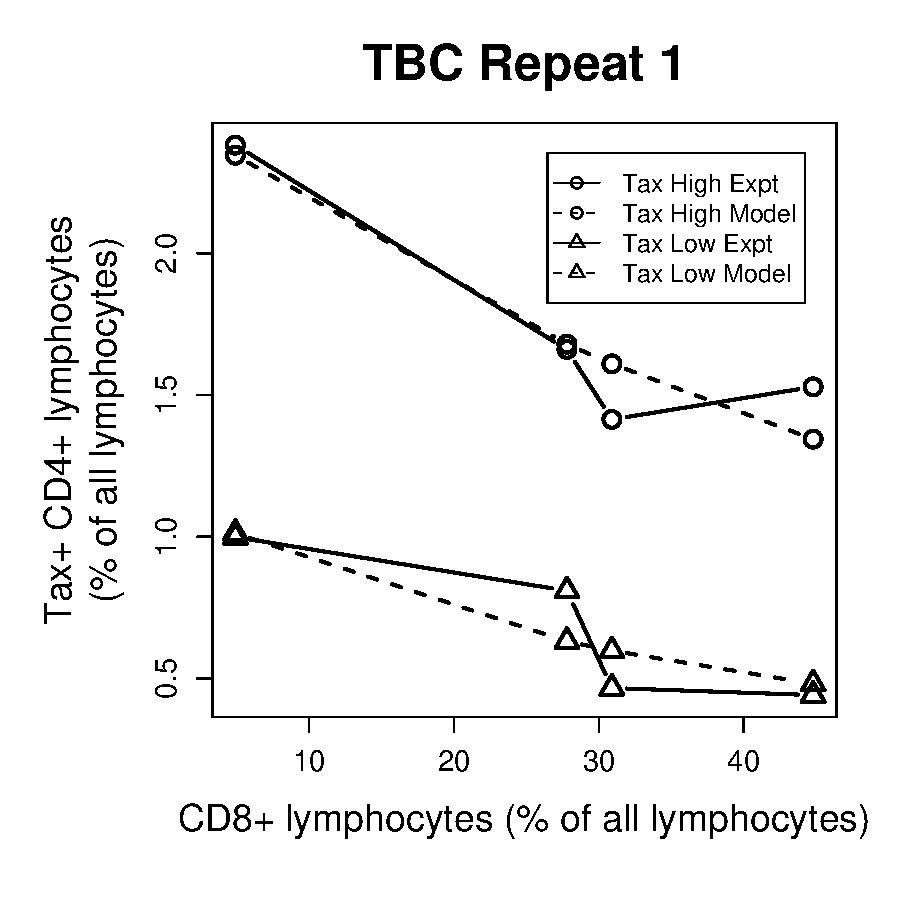
\includegraphics[width=7cm]{./Figures/chapter5/figure_lysis_tbc_rep_1}%
\hspace{0cm}%
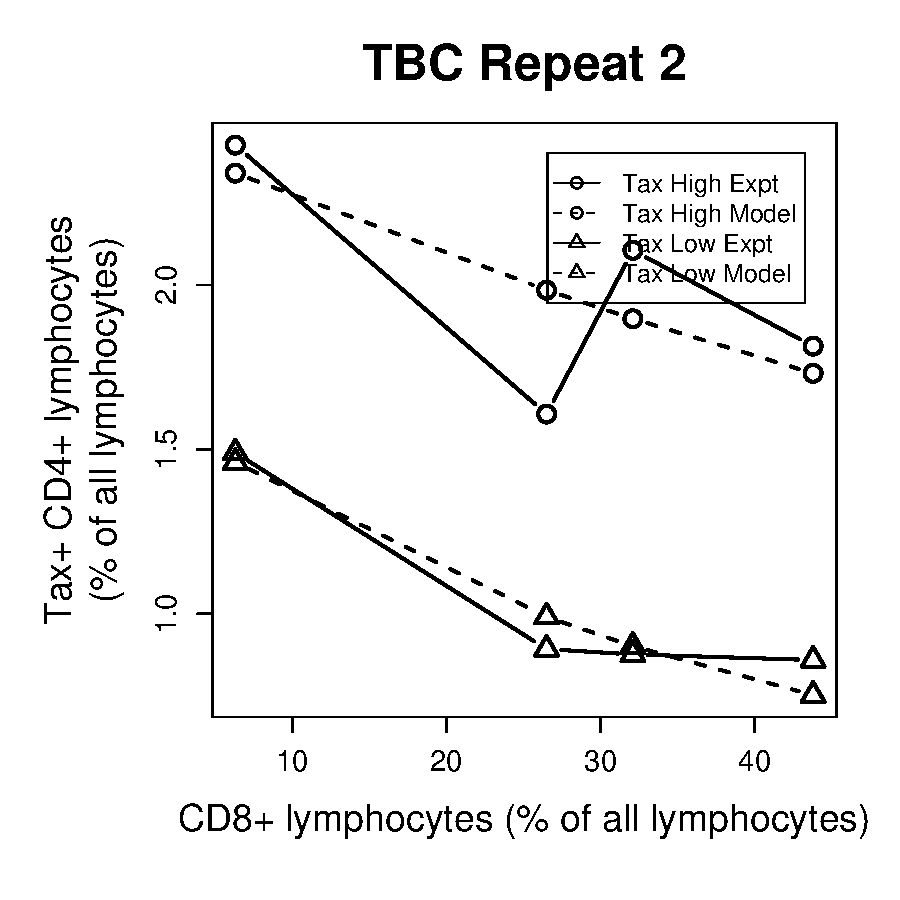
\includegraphics[width=7cm]{./Figures/chapter5/figure_lysis_tbc_rep_2} \\
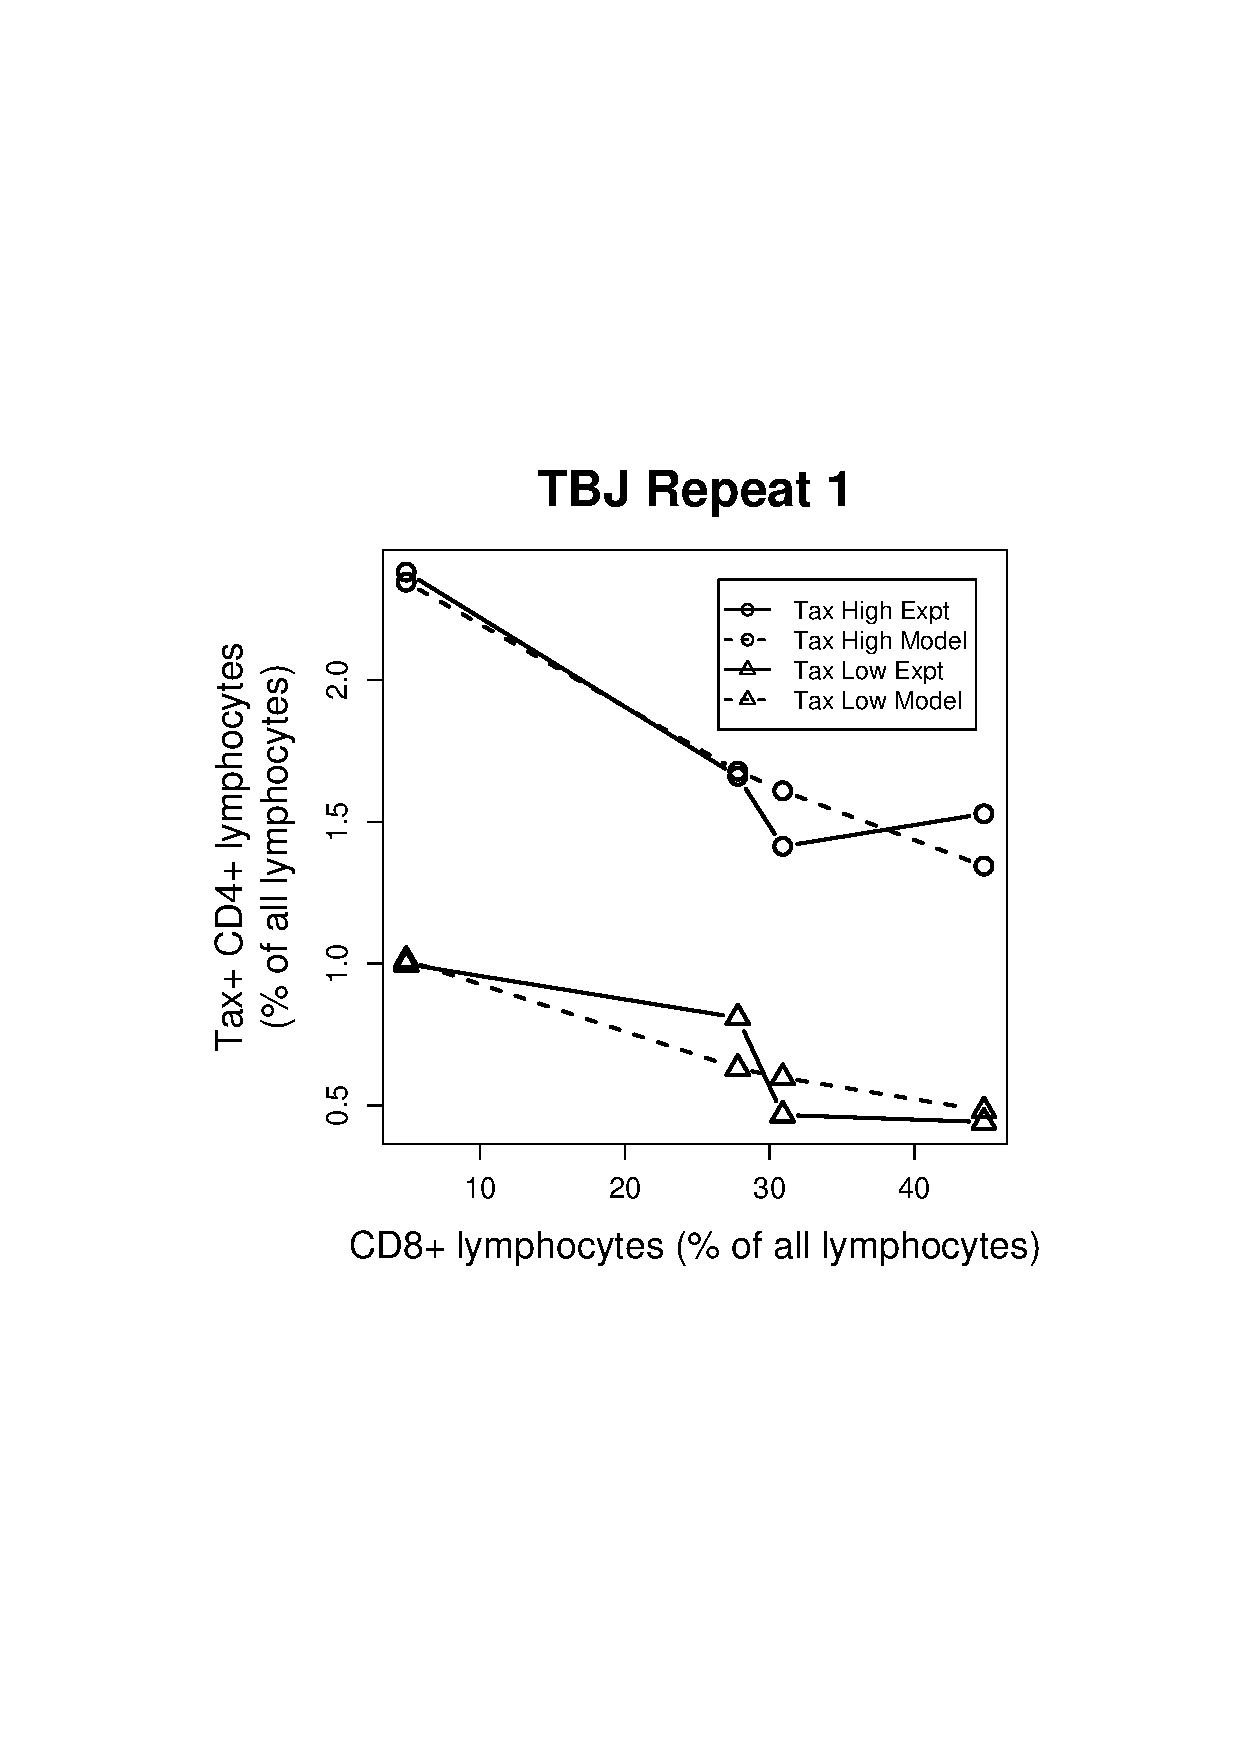
\includegraphics[width=7cm]{./Figures/chapter5/figure_lysis_tbj_rep_1}%
\hspace{0cm}%
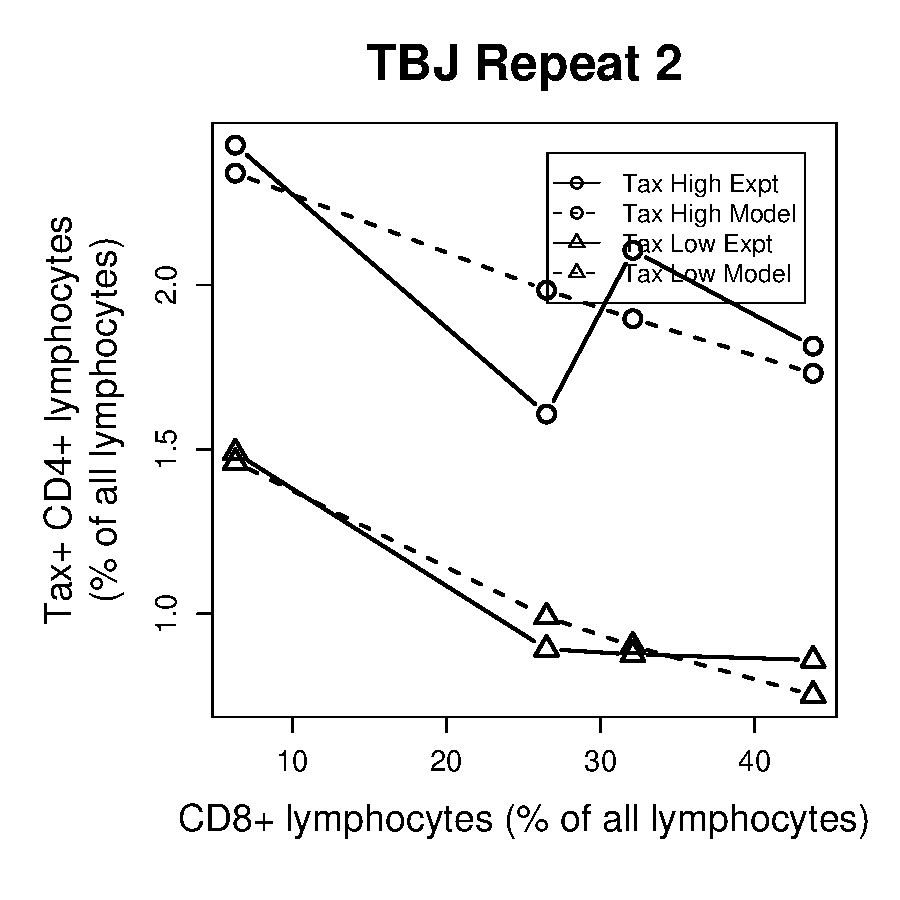
\includegraphics[width=7cm]{./Figures/chapter5/figure_lysis_tbj_rep_2} \\
\contcaption{Continued}
\end{figure}

\begin{figure}[htp]
\centering
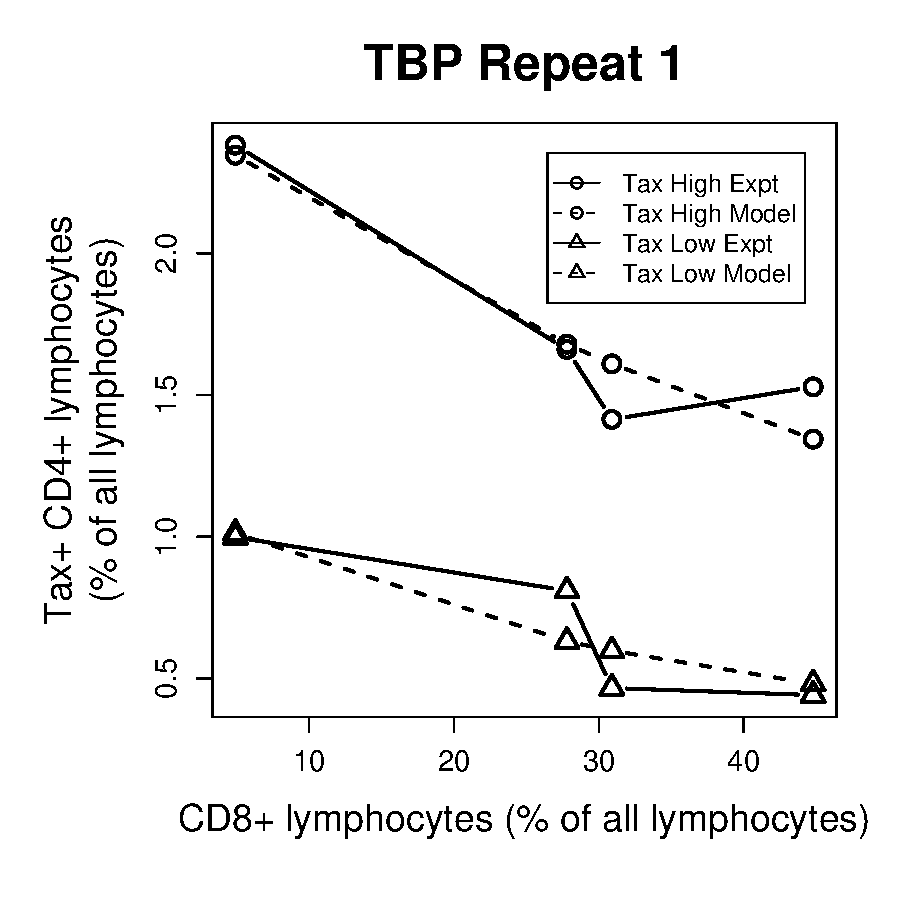
\includegraphics[width=7cm]{./Figures/chapter5/figure_lysis_tbp_rep_1}%
\hspace{0cm}%
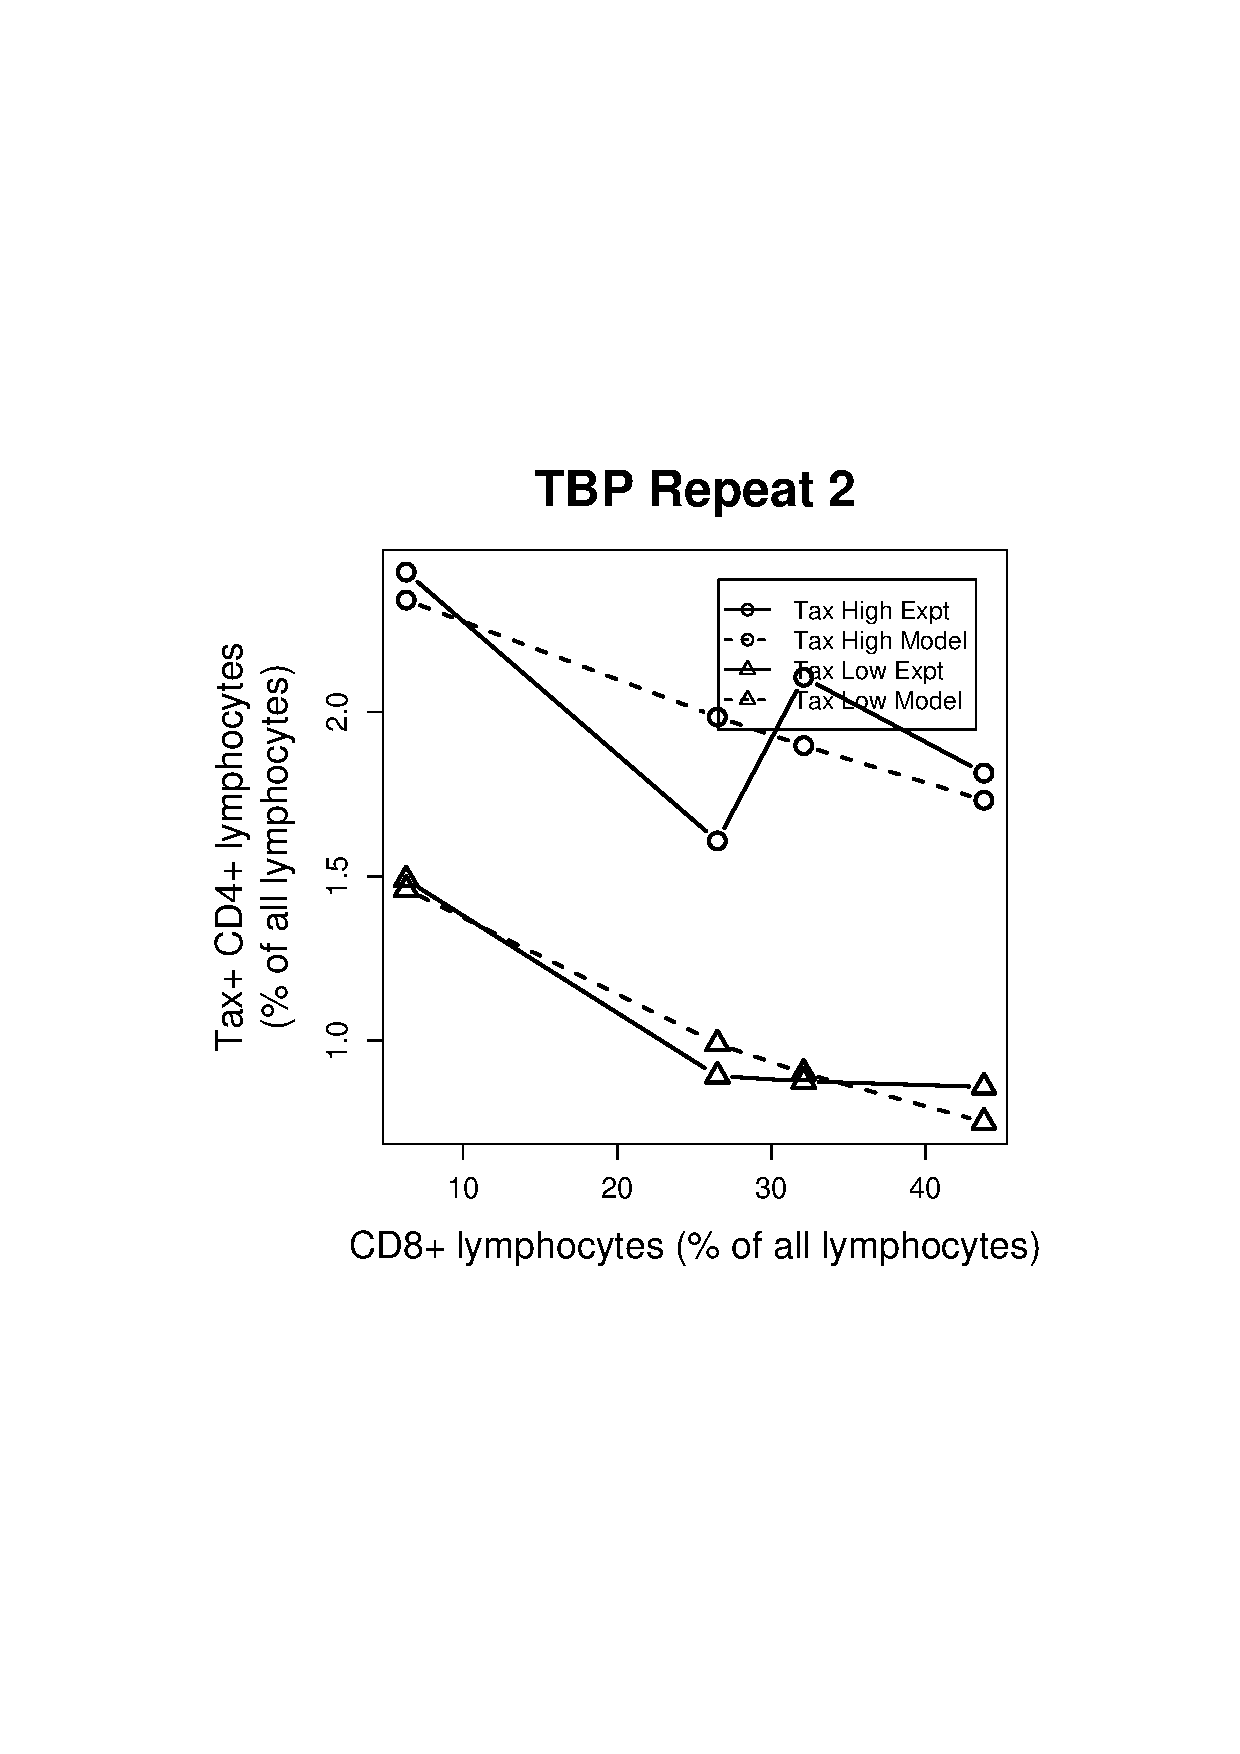
\includegraphics[width=7cm]{./Figures/chapter5/figure_lysis_tbp_rep_2} \\
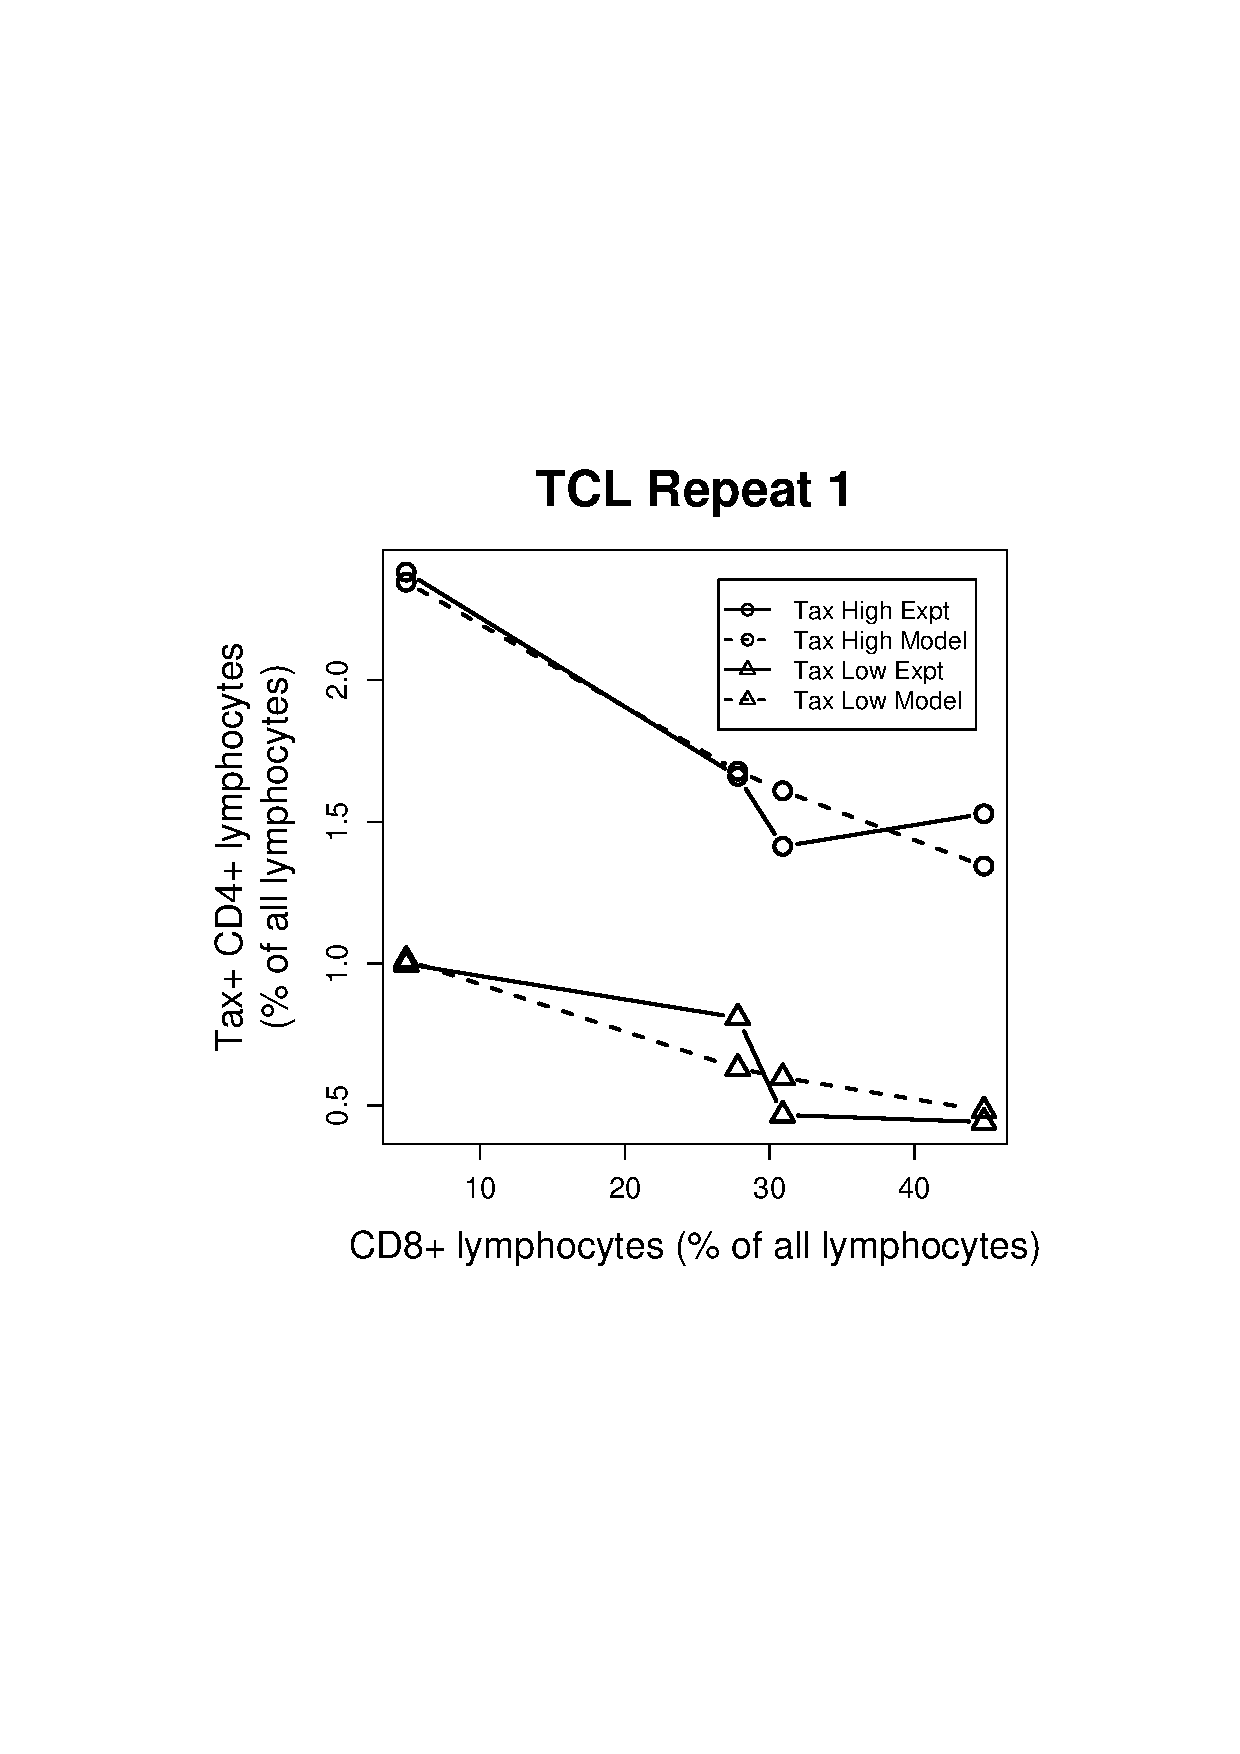
\includegraphics[width=7cm]{./Figures/chapter5/figure_lysis_tcl_rep_1}%
\hspace{0cm}%
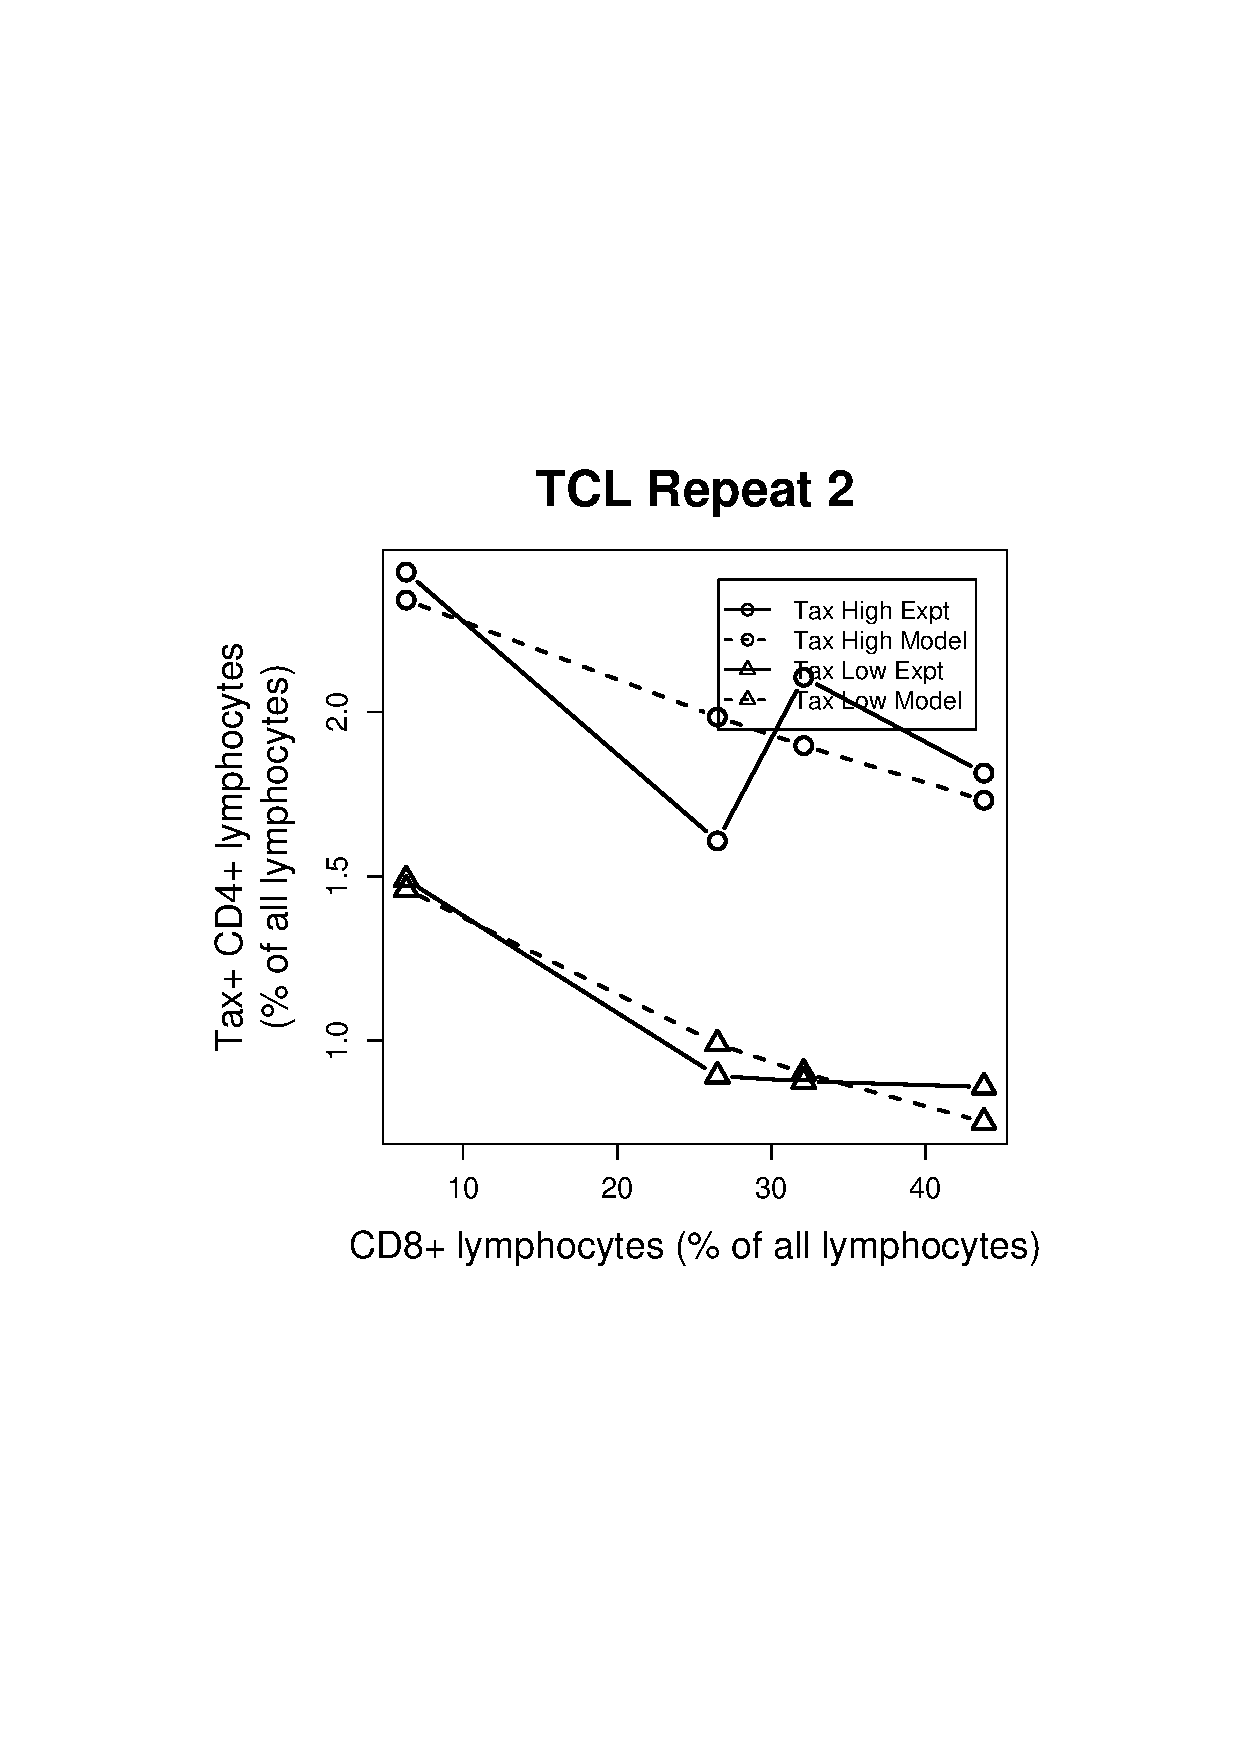
\includegraphics[width=7cm]{./Figures/chapter5/figure_lysis_tcl_rep_2} \\
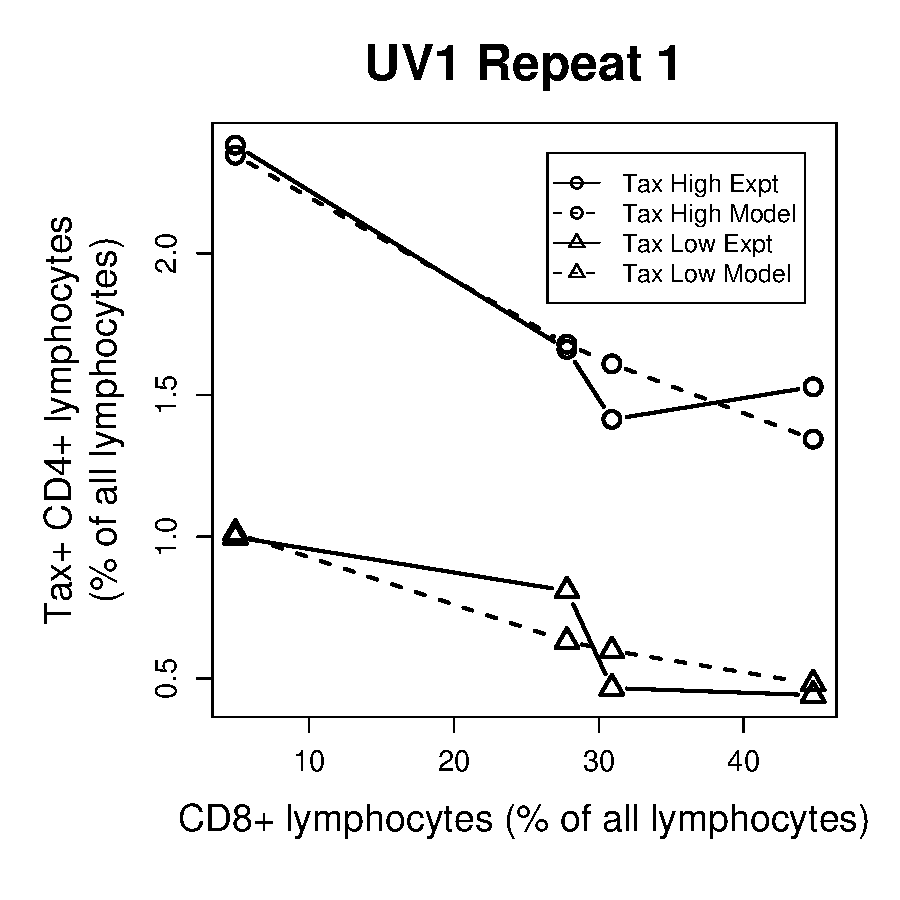
\includegraphics[width=7cm]{./Figures/chapter5/figure_lysis_uv1_rep_1}%
\hspace{0cm}%
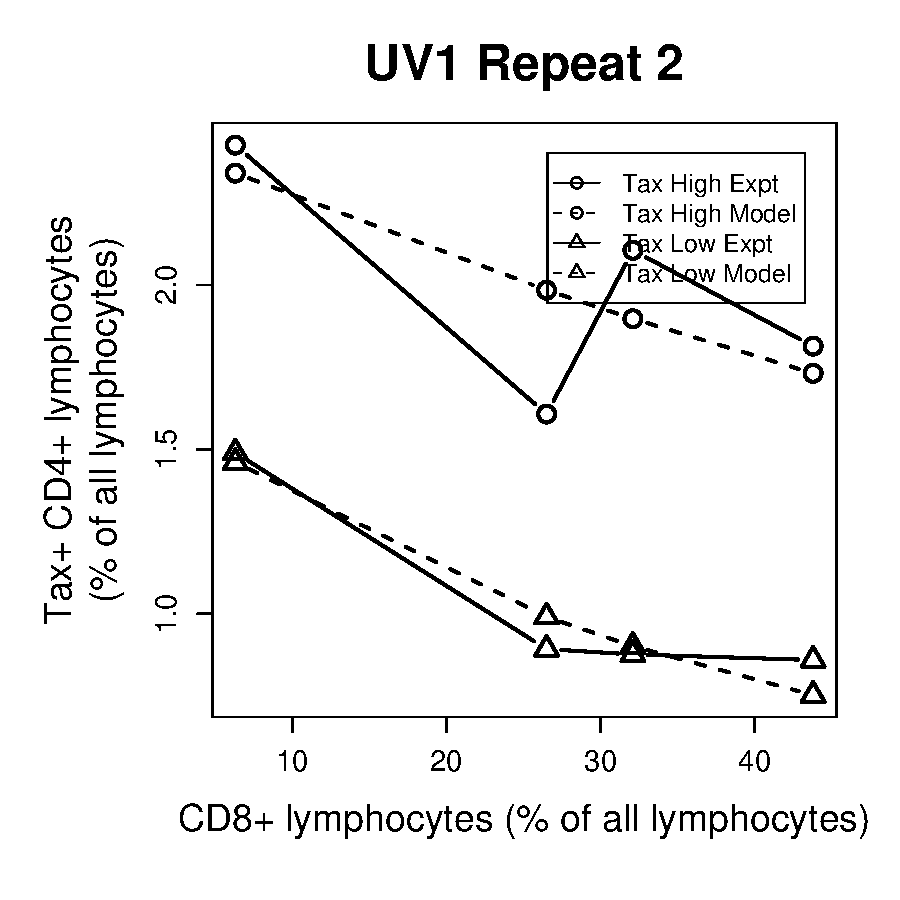
\includegraphics[width=7cm]{./Figures/chapter5/figure_lysis_uv1_rep_2} \\
\contcaption{Continued}
\end{figure}

%%%%%%%%%%%%%%%%%%%%%%%%%%%%%%%%%%%%%%%%%%%%%%%%%%%%%%%%%%%%%%%%%%%%%%%%%%%%%%%%%%%%%%%%%%%%%%%%%%%%

\begin{figure}[htp]
\centering
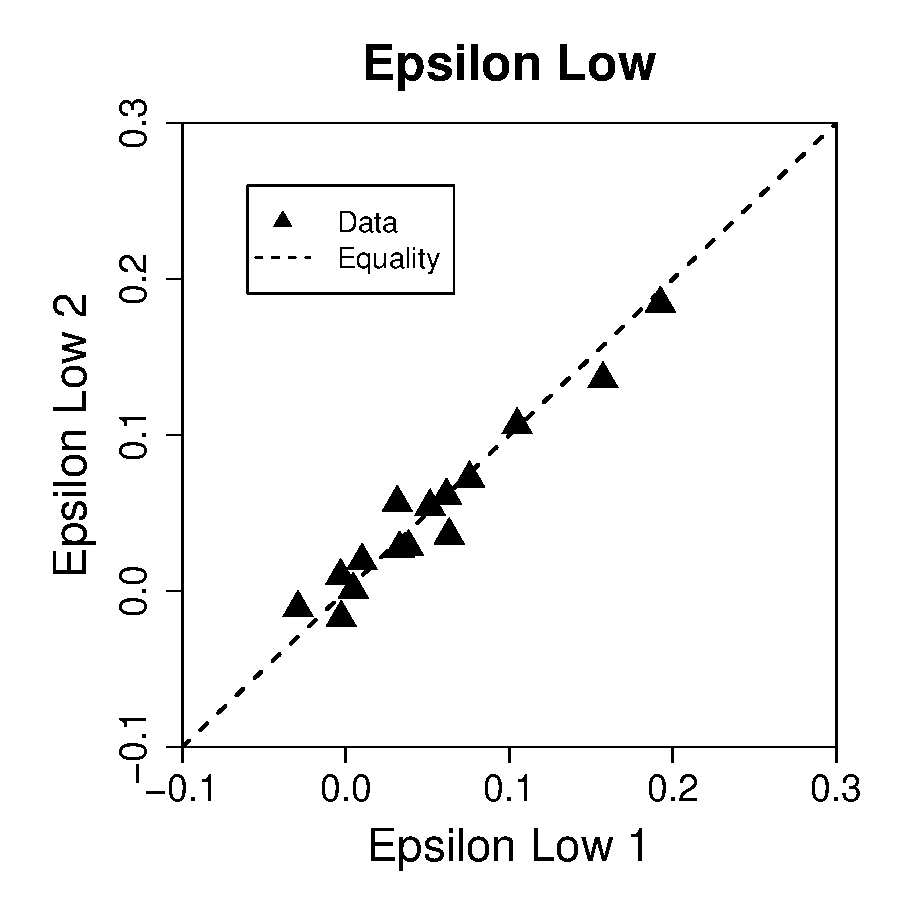
\includegraphics[width=7cm]{./Figures/chapter5/figureLowReps}%
\hspace{0cm}%
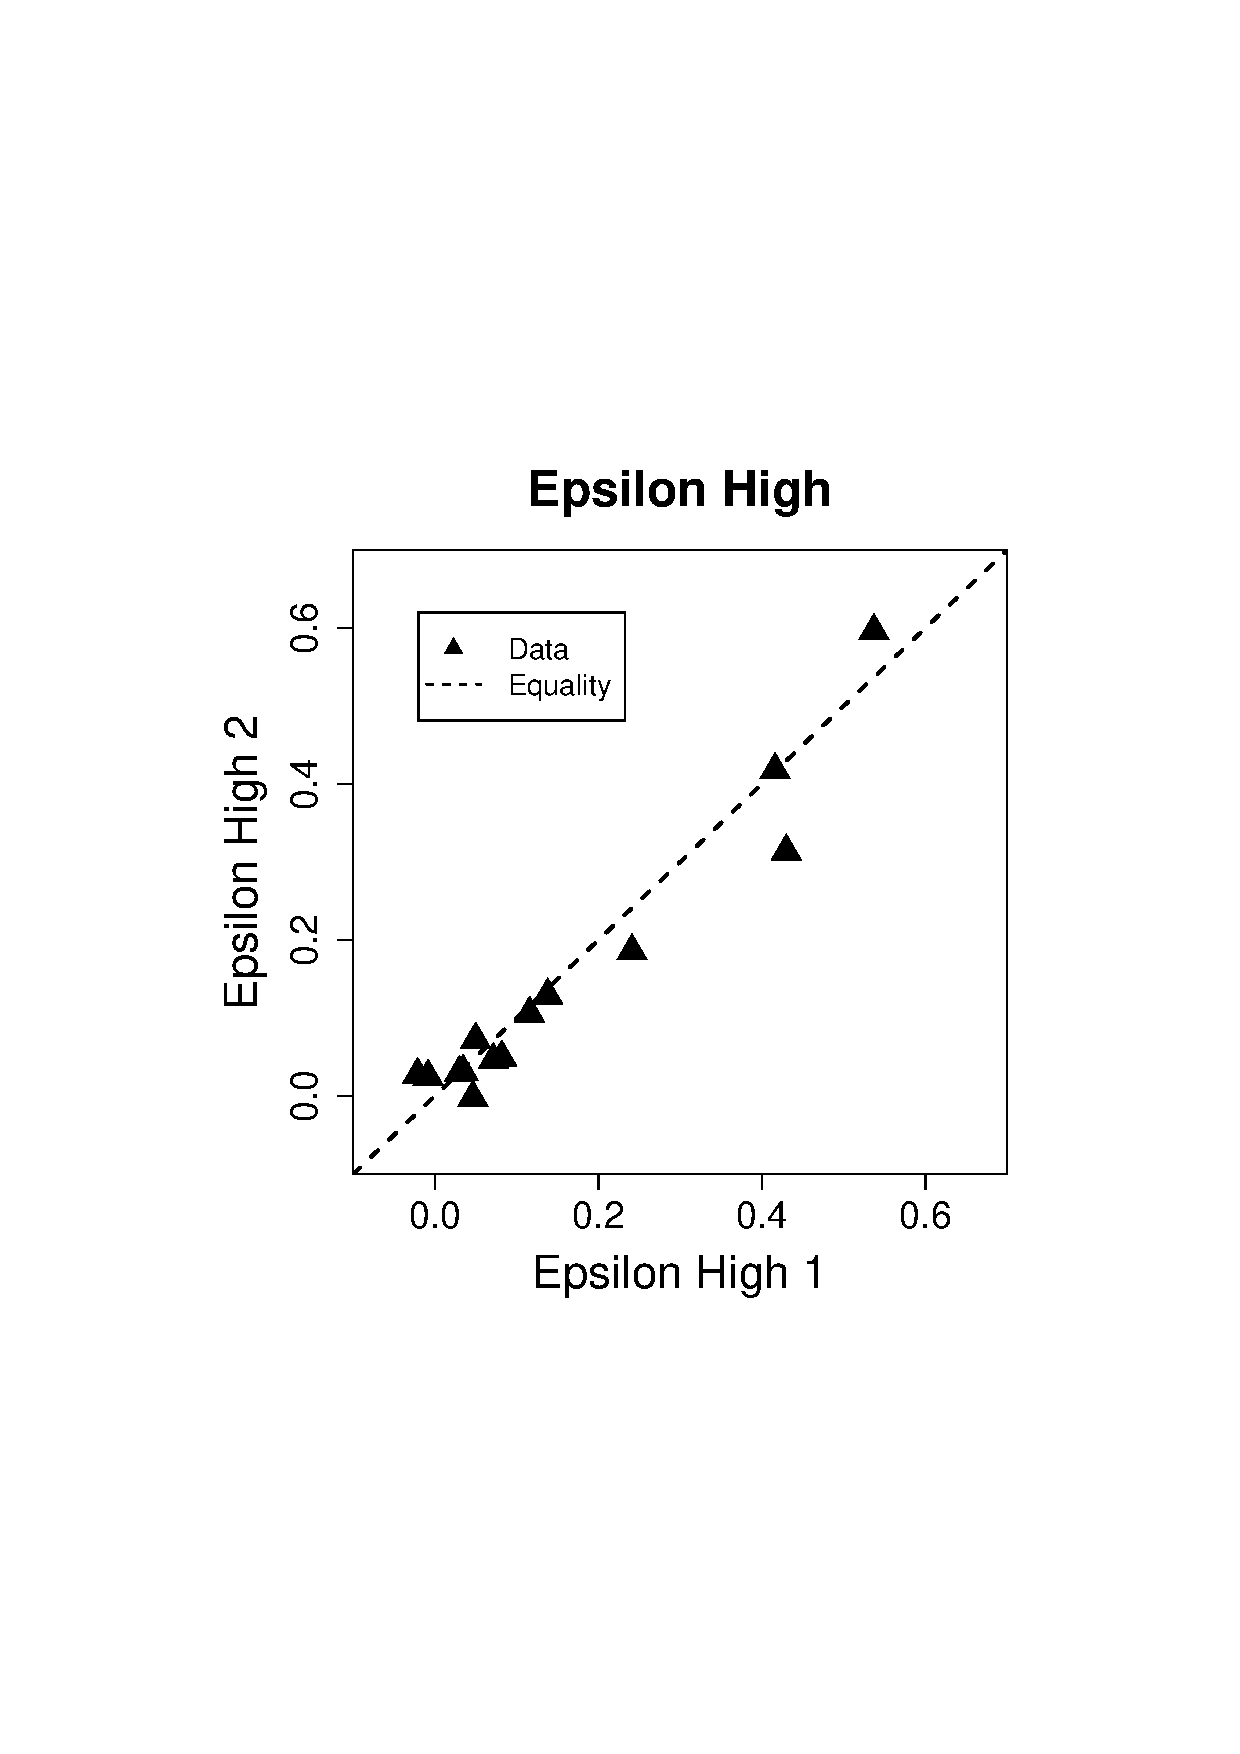
\includegraphics[width=7cm]{./Figures/chapter5/figureHighReps} \\
\caption[A comparison of repeat measures of $\epsilon$\superscript{low} and $\epsilon$\superscript{high}]{A comparison of repeat measures of $\epsilon$\superscript{low} and $\epsilon$\superscript{high}. Both showed high agreement across repeats ($\epsilon$\superscript{low}: $R^2 = 0.9492$, $P < 0.001$. $\epsilon$\superscript{high}: $R^2 = 0.890$, $P < 0.001$).}
\label{appendixb/figure1}
\end{figure}

\begin{figure}[htp]
\centering
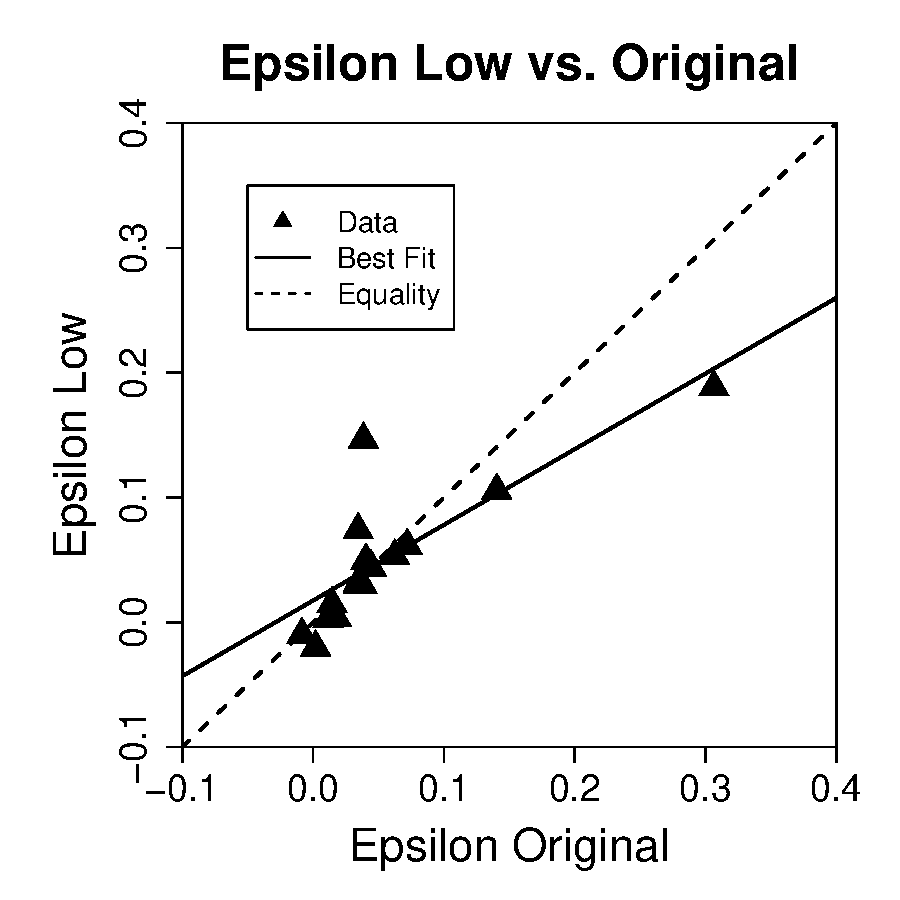
\includegraphics[width=7cm]{./Figures/chapter5/figureLowOrig}%
\hspace{0cm}%
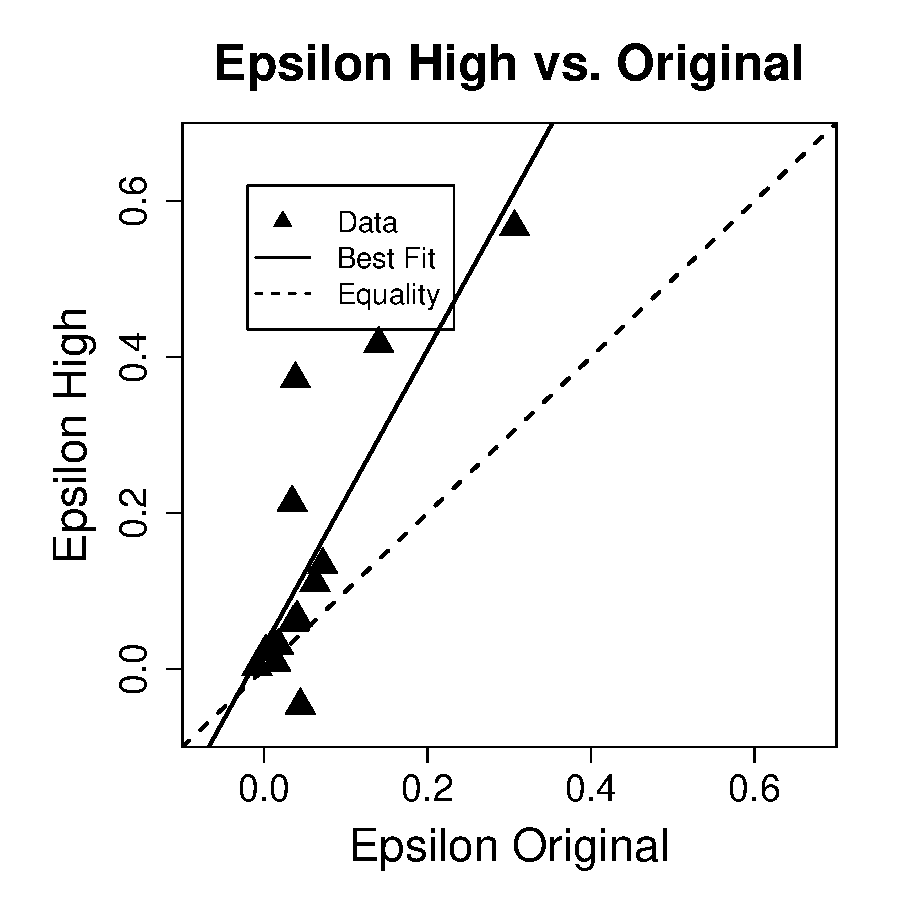
\includegraphics[width=7cm]{./Figures/chapter5/figureHighOrig} \\
\caption[A comparison of parameter $\epsilon$ with $\epsilon$\superscript{low} and $\epsilon$\superscript{high}]{A comparison of parameter $\epsilon$ with $\epsilon$\superscript{low} and $\epsilon$\superscript{high}. The killing rate $\epsilon$ of the original lysis model \eref{chapter5/equation1} compared to $\epsilon$\superscript{high} ($R^2 = 0.686$, $P < 0.001$) and $\epsilon$\superscript{low} ($R^2 = 0.658$, $P < 0.001$).}
\label{appendixb/figure2}
\end{figure}

\begin{figure}[htp]
\centering
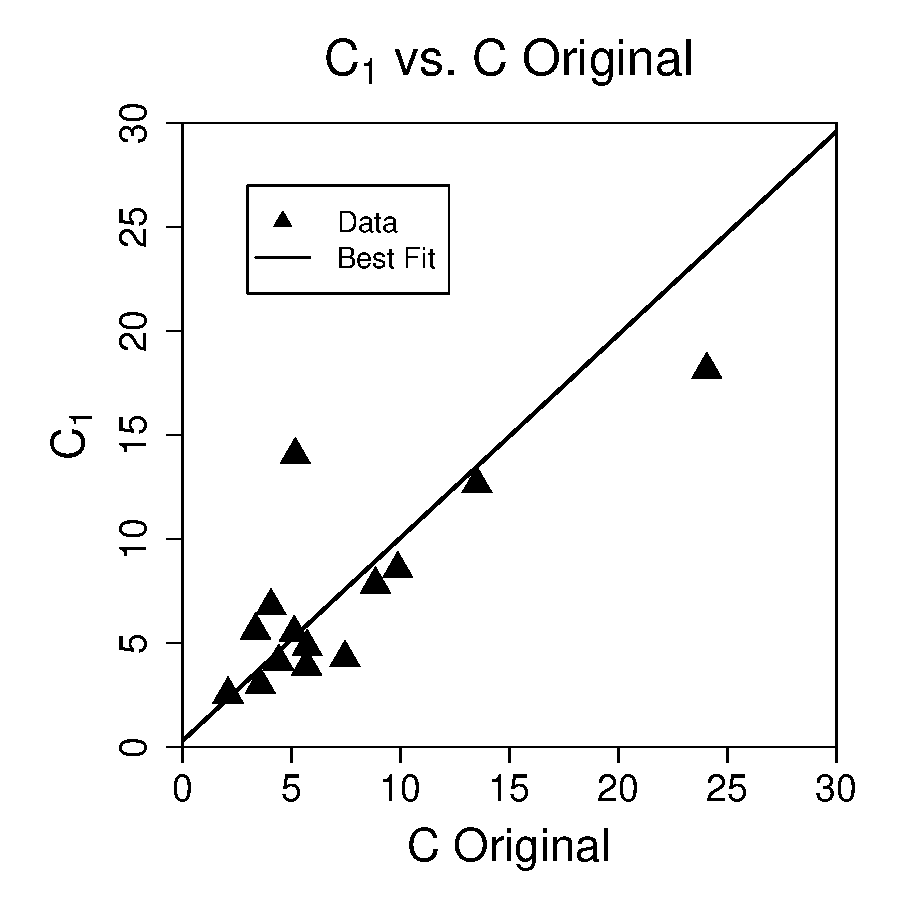
\includegraphics[width=7cm]{./Figures/chapter5/figurec1cOrig}%
\hspace{0cm}%
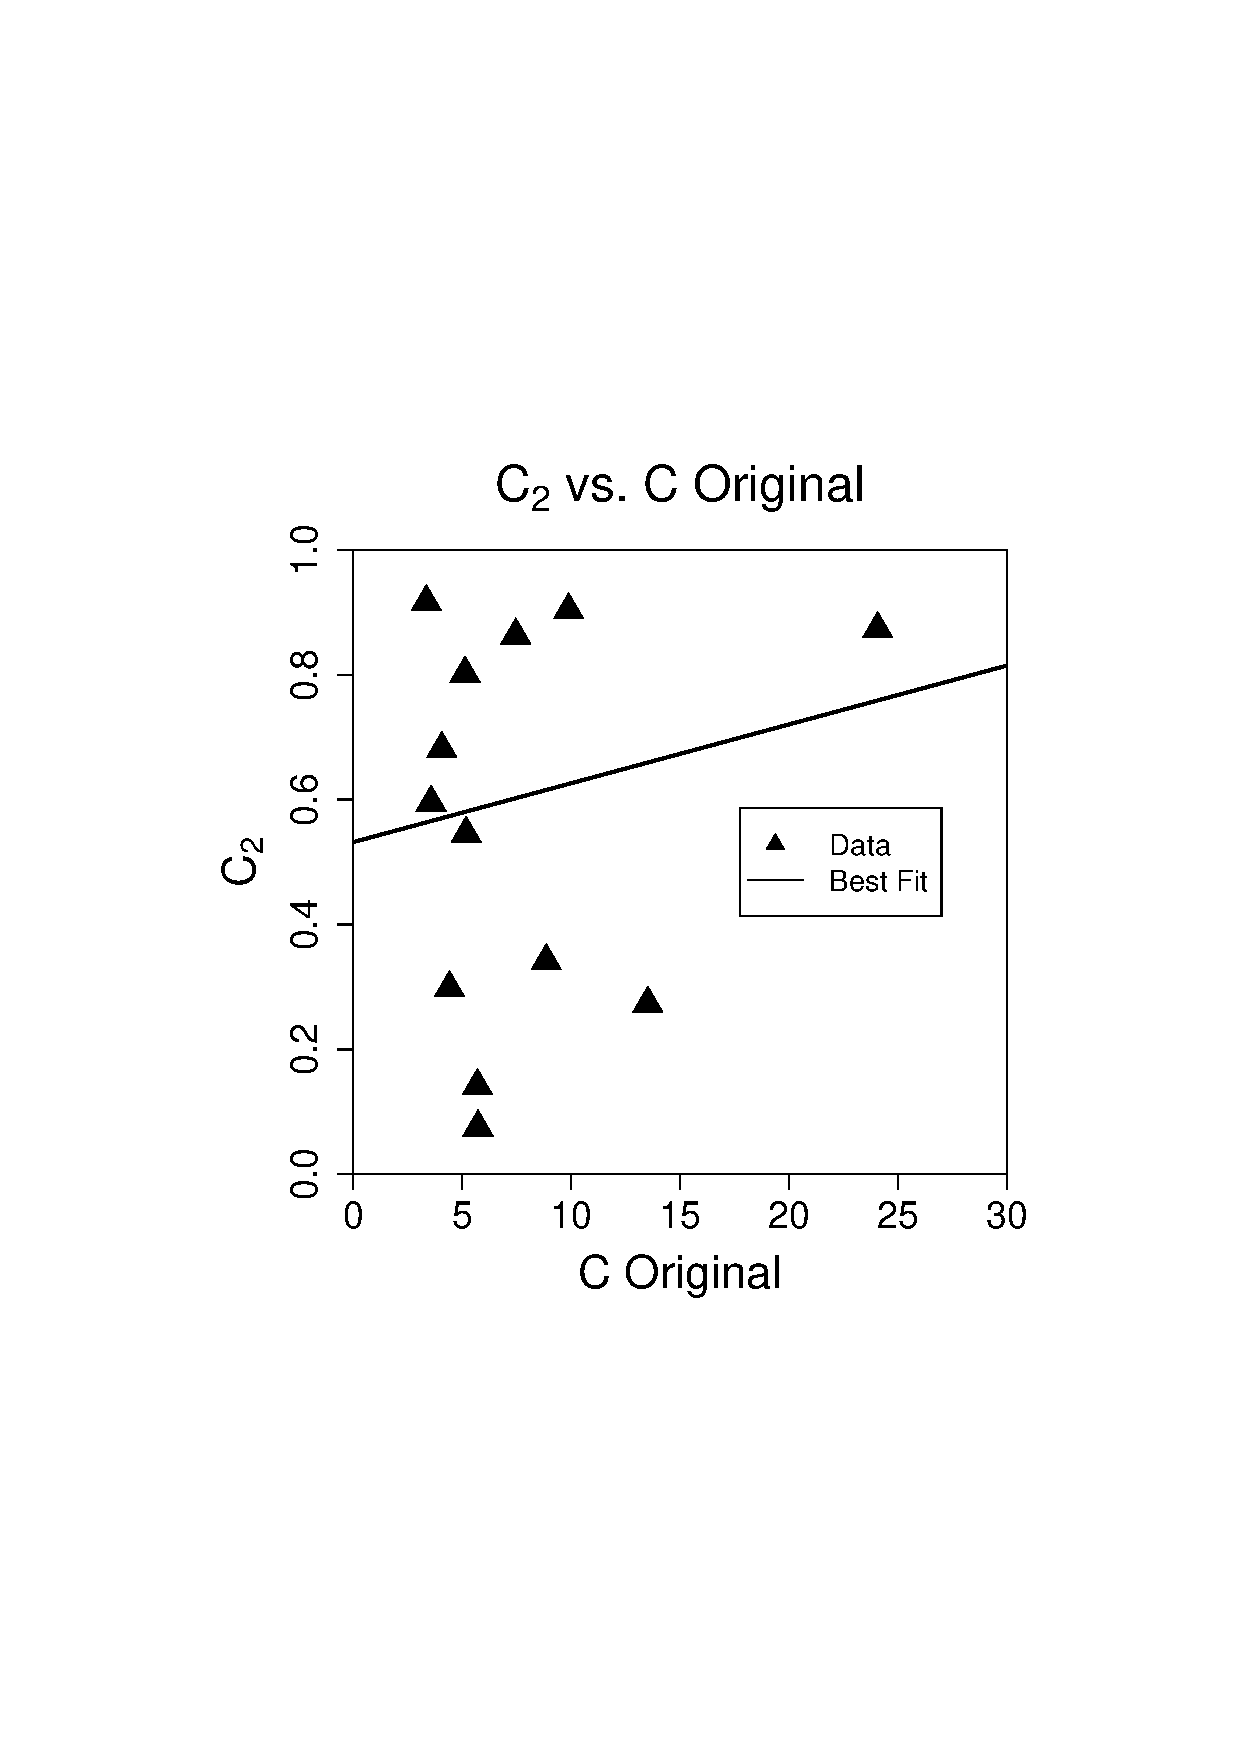
\includegraphics[width=7cm]{./Figures/chapter5/figurec2cOrig} \\
\caption[A comparison of parameter $c$ with $c_1$ and $c_2$]{A comparison of parameter $c$ with $c_1$ and $c_2$. The parameter $c$ of the original lysis model \eref{chapter5/equation1} compared to the rate of increase of Tax\superscript{low} $c_1$ ($R^2 = 0.934$, $P < 0.001$) and Tax\superscript{high} $c_2$ ($R^2 = 0.129$, $P = 0.189$).}
\label{appendixb/figure3}
\end{figure}

\begin{figure}[htp]
\centering
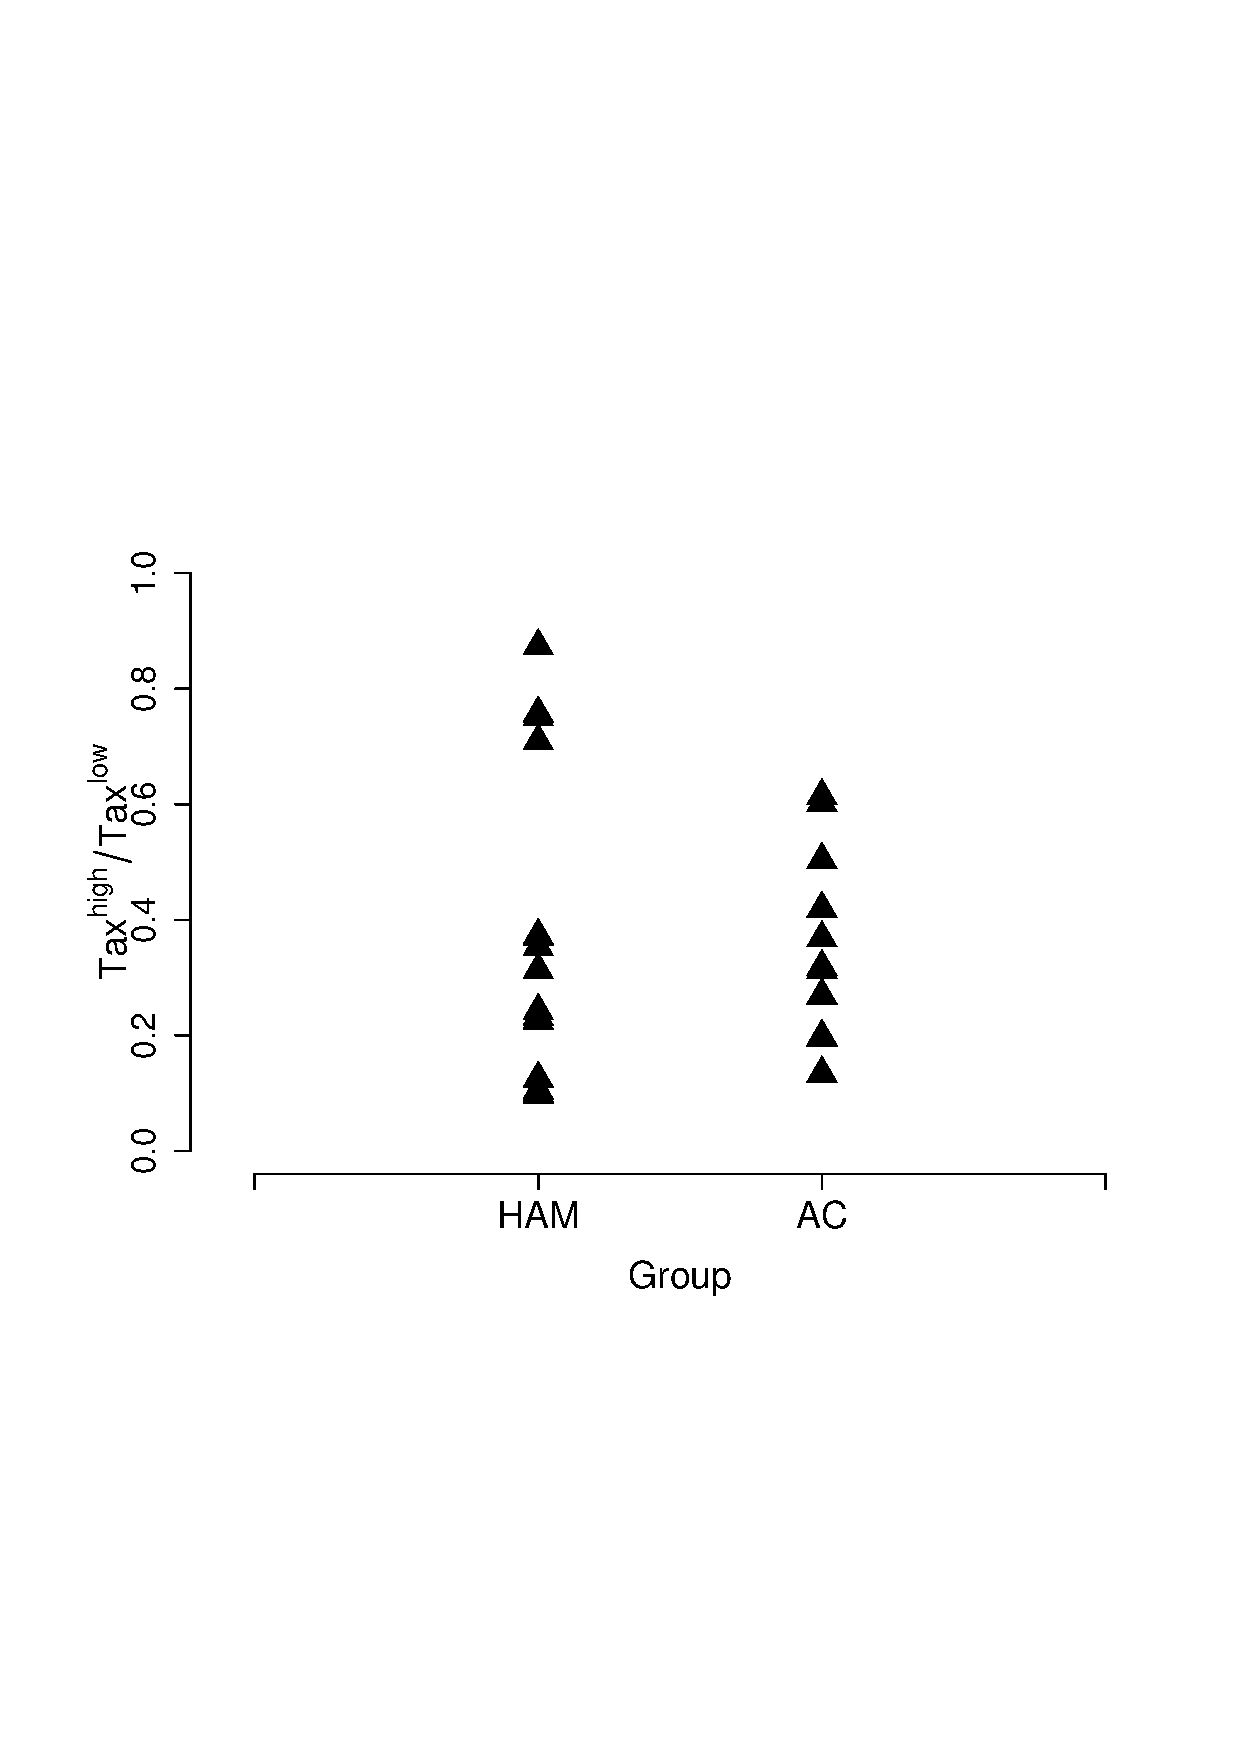
\includegraphics[width=14cm]{./Figures/chapter5/Ratios}
\caption[The ratio of Tax expression for HAM/TSP and AC patients]{The ratio of Tax expression for HAM/TSP and AC patients. We found no difference in the Tax\superscript{high}/Tax\superscript{low} ratio between 8 HAM/TSP patients and 6 AC patients ($P = 0.871$, Wilcoxon-Mann-Whitney, HAM/TSP: $n=16$, AC: $n=12$). Both repeats for each patient were used.}
\label{chapter5/figureRatio}
\end{figure}